\chapter{Python Static Analysis based on Abstract Interpretation}%
\label{appendix-ai-theory}

This appendix is divided into two parts: first, we present a reduced set of the Python
syntax together with a (partial) operational semantics; second, we show the use of the
formal semantic definition to define the abstract interpretation solution we implemented.

This chapter is meant to explain the theory behind the Abstract Interpreter implemented.
In Chapter~\ref{pytropos-analysis-implementation} an explanation on the implementation
details is given.

\section{Python (reduced) syntax and semantics}

Python has no official small-step (formal) semantics. The Python Software Foundation
defines a Reference Manual for the language
\autocite{python_software_foundation_python_2019}, but they are explicit that the manual
does not define a full specification for the language. Quote: \enquote{\ldots{} if you
were coming from Mars and tried to re-implement Python from this document alone, you might
have to guess things and in fact, you would probably end up implementing quite a different
language.}

There have been a couple of small-step semantics defined for Python
\autocites{politz_python_2013}{fromherz_static_2018}{guth_formal_2013}{ranson_semantics_2008}.
In this work, we define yet one more time small-step semantics for Python. We decided to
define our small-step semantics for Python because of our specific needs.

Our semantics definition resembles the most that of \textcite{fromherz_static_2018}. In
fact, our
definition is loosely based on \textcite{fromherz_static_2018}. As Fromherzet.~al, we
define each expression and statement step as a function from states to states of the
program, but opposed to them we do not include exception handling and control break statements.
Our definition allows every single value in the language to be an object: functions,
attributes, subscripts, and primitive values are all objects just as in regular Python.
The following is valid in Python and in our definition:

\begin{pythoncode}
a = []
b = a.append
b(3)
a.append(2.0)
print(a)  # prints: [3, 2.0]
\end{pythoncode}

In this sense, our definition is closer to that of \textcite{politz_python_2013}, where
they also show how their semantics are able to handle similarly complex examples.

\subsection{(Reduced) Syntax}\label{reduced-syntax}

Our simplified version of Python's Syntax can be seen in Figure~\ref{syntaxPythonAppen}.
Modified from AST's syntax below from Figure~\ref{syntaxPython2App}.

% {\inlinetodo{Translate into LaTeX equations}}

\begin{figure}
\[\begin{array}{rclr}
    expr  &:=& i \in \mathbb{Z} \alt j \in \texttt{float} \alt \texttt{True} \alt
    \texttt{False} \alt \texttt{None} & \textit{primitive values} \\
     &\alt& identifier & \textit{variable name} \\
     %&\alt& \texttt{Undefined} & \textit{wildcard value} \\
     &\alt& expr~op~expr \alt expr~cmpop~expr & \textit{binary operations} \\
     &\alt& expr\texttt{(}expr*\texttt{)}     & \textit{function call} \\
     &\alt& expr\texttt{.}identifier & \textit{attribute access} \\
     &\alt& expr\texttt{[}expr\texttt{]}      & \textit{subscript access} \\
     &\alt& \texttt{[}expr*\texttt{]}         & \textit{lists} \\
     &\alt& \texttt{(}expr*\texttt{)}         & \textit{tuples} \\

  stmt &:=& \texttt{del } expr  & \textit{delete} \\
     &\alt& expr = expr         & \textit{assignment} \\
     &\alt& expr~op\hspace{-0.35em}\texttt{ = } expr       & \textit{augmented assignment} \\
     &\alt& expr\texttt{: } expr \texttt{ = } expr         & \textit{type annotation} \\
     &\alt& \texttt{while } expr\texttt{: } stmt^+         & \textit{loop} \\
     &\alt& \texttt{if } expr\texttt{: } stmt^+ \texttt{ else: } stmt^+  & \textit{if-else} \\
     &\alt& \texttt{import } alias^+
     \alt \texttt{from } identifier \texttt{ import } alias^+   & \textit{import library} \\
     &\alt& expr & \\

  op &:=& \texttt{+} \alt \texttt{-} \alt \texttt{*} \alt \texttt{/} \alt \texttt{\%} \alt \texttt{**} \alt
      \texttt{<<} \alt \texttt{>>} \alt \texttt{//}  & \\
  cmpop &:=& \texttt{<} \alt \texttt{<=} \alt \texttt{>} \alt \texttt{>=}  & \\

  alias &:=& identifier \alt identifier \texttt{ as } identifier  & \\

  %identifier &:=& str  & \\
\end{array}\]
\caption{Reduced Python syntax used throughout this work.\label{syntaxPythonAppen}}
\end{figure}

%\begin{verbatim}
%mod = stmt*  -- A program. Starting point
%
%expr = Int(i) for i \in \N | Float(j) for j \in floats
%     | True | False | None
%
%     | identifier         -- variable name
%
%     | expr op expr       -- eg, a + 5
%     | expr cmpop expr    -- eg, a < 5
%     | expr(expr*)        -- Function calling
%
%     | expr.identifier    -- Attribute access
%     | expr[expr]         -- Not supported for NumPy Arrays :S
%     | [expr*]            -- list
%     | (expr*)            -- tuple
%
%stmt = del expr           -- delete expression
%      | expr = expr       -- assignment
%      | expr op= expr     -- augmented assignment
%      | expr: expr = expr -- type annotation
%      | while expr: stmt+
%      | if expr: stmt+
%      | import alias+
%      | from identifier import alias+
%      | expr              -- An expression can be an statement
%
%op = + | - | * | / | % | ** | << | >> | //
%cmpop = < | <= | > | >=
%
%alias = identifier | identifier as identifier
%
%identifier = string  -- with some restrictions
%\end{verbatim}

The syntax from Figure~\ref{syntaxPythonAppen} is a subset of the Python 3.6 syntax\footnote{%
  Modified from the Python 3.6 syntax found at
  \url{https://github.com/python/typed_ast/blob/89242344f18f94dc109823c0732325033264e22b/ast3/Parser/Python.asdl}
}. Note that CPython does not directly interpret code written in this syntax. The usual
steps of lexing and parsing into a more explicit representation are necessary for a
program to be executed by CPython. We will define the semantics of the language over the
parser's syntax, see Figure~\ref{syntaxPython2App} and not over the aforementioned syntax. The reasoning behind this change
is due to the parser's syntax readiness to be analysed opposed to the original syntax.

\begin{figure}
\[\begin{array}{rclr}
    expr  &:=& \texttt{Int(}i\texttt{)} \textit{ for } i \in \mathbb{Z}
          \alt \texttt{Float(}j\texttt{)} \textit{ for } j \in \texttt{float} \\
          &\alt& \texttt{True}
          \alt \texttt{False} \alt \texttt{None}   & \textit{primitive values} \\
     &\alt& \SLit{Name}{identifier, expr\_context} & \textit{variable name} \\
     %&\alt& \texttt{Undefined} & \textit{wildcard value} \\
     &\alt& \SLit{BinOp}{op, expr, expr} \\
     &\alt&   \SLit{Compare}{expr, cmpop, expr}             & \textit{binary operations} \\
     &\alt& \SLit{Call}{expr, expr*}                    & \textit{function call} \\
     &\alt& \SLit{Attribute}{expr, identifier}          & \textit{attribute access} \\
     &\alt& \SLit{Subscript}{expr, expr, expr\_context} & \textit{subscript access} \\
     &\alt& \SLit{List}{expr*}                          & \textit{lists} \\
     &\alt& \SLit{Tuple}{expr*}                         & \textit{tuples} \\

  stmt &:=& \SLit{Delete}{expr}                      & \textit{delete} \\
     &\alt& \SLit{Assign}{expr, expr}              & \textit{assignment} \\
     &\alt& \SLit{AugAssign}{expr, op, expr}       & \textit{augmented assignment} \\
     &\alt& \SLit{AnnAssign}{expr, expr, expr}     & \textit{type annotation} \\
     &\alt& \SLit{While}{expr, stmt^+}             & \textit{loop} \\
     &\alt& \SLit{If}{expr, stmt^+, stmt^+}        & \textit{if} \\
     &\alt& \SLit{Import}{alias^+}                 & \textit{import library} \\
     &\alt& \SLit{ImportFrom}{identifier, alias^+} & \textit{import from} \\
     &\alt& \SLit{Expr}{expr}                      & \\

  expr\_context &:=& \SLoad \alt \SStore \alt \SDel  & \\

  op &:=& \texttt{Add} \alt \texttt{Sub} \alt \texttt{Mult} \alt \texttt{Div} \alt
         \texttt{Mod} \alt \texttt{Pow} \\
     &\alt& \texttt{LShift} \alt \texttt{RShift} \alt \texttt{FloorDiv}  & \\
  cmpop &:=& \texttt{Lt} \alt \texttt{LtE} \alt \texttt{Gt} \alt \texttt{GtE}  & \\

  alias &:=& identifier \alt (identifier, identifier) & \\

  %identifier &:=& str  & \\
\end{array}\]
\caption{Python syntax used to define the semantics of the Abstract
  Interpreter.\label{syntaxPython2App}}
\end{figure}

%\begin{verbatim}
%mod = Module(stmt* body)
%
%expr = Int(n)
%     | Float(n) | True | False | None
%     | Name(identifier, expr_context)
%     | BinOp(operator, expr, expr)
%     | Compare(expr, cmpop, expr)
%     | Call(expr, expr*)
%     | Attribute(expr, identifier)
%     -- No need for expr_context because no user made objects are allowed yet, thus
%     -- modifying attributes is not necessary
%     -- | Attribute(expr, identifier, expr_context)
%     | Subscript(expr, expr, expr_context)  -- No arbitrary slice allowed yet
%     | List(expr*)
%     | Tuple(expr*) -- No expr_context for Tuple as `(a, b) = 1, 2` is not supported
%
%stmt = Delete(expr+)
%      | Assign(expr, expr)                -- a = 3
%      | AugAssign(expr, operator, expr)   -- a += 3
%      | AnnAssign(expr, expr, expr)       -- a: int = 3
%
%      | While(expr, stmt+)
%      | If(expr, stmt+, stmt*)
%
%      | Import(alias+ names)
%      | ImportFrom(identifier, alias+)
%
%      | Expr(expr)
%
%-- Indicates why are we looking up a variable, attribute or subscript
%expr_context = Load | Store | Del
%
%operator = Add | Sub | Mult | Div | Mod | Pow | LShift
%             | RShift | FloorDiv
%
%cmpop = Lt | LtE | Gt | GtE
%
%-- import name with optional 'as' alias.
%alias = (identifier, identifier?)
%\end{verbatim}

Code written in the subset of Python (Figure~\ref{syntaxPythonAppen}) gets translated into
the parser's representation (Figure~\ref{syntaxPython2App}), over which we define the
semantics of the language. We will no describe the process of translation (parsing), but
we will explore some examples to show why the parser's syntax aids into the definition of
the small-step semantics:

\begin{itemize}
\item \pycode|a + b| gets translated into
  \pycode|BinOp(Add, Name(a, Load), Name(b, Load))|. Notice the \pycode|Load| context, it
  indicates that we want to get the value of the variable, not a reference to it.
\item \pycode|a = 3| gets translated into
  \pycode|Assign(Name(a, Store), Int(3))|. Notice the \pycode|Store|
  context, it tells us that we want to modify the variable \pycode|a|, i.e. we want a
  reference to the variable.
\item
  \pycode|del a| gets translated into \pycode|Delete(Name(a, Del))|.
  Notice the \pycode|Del| context, it tells us that we will where the object location in
  the heap.
\item
  \pycode|a.b[3] + b.c| gets translated into

\begin{pythoncode}
BinOp(Add,
  Subscript(Attribute(Name(a, Load), b), Int(3), Load),
  Attribute(Name(b, Load), c)
)
\end{pythoncode}
\item
  \pycode|a.b[3] = 3| gets translated into

\begin{pythoncode}
Assign(
  Subscript(Attribute(Name(a, Load), b), Int(3), Store),
  Int(3)
)
\end{pythoncode}

  Notice how we only get the \pycode|Store| context for the subscript
  and not for anything else, as we only want to know where the value of
  the subscript is stored.
\item
  \pycode|del a.b[3]| gets translated into

\begin{pythoncode}
Delete(
  Subscript(Attribute(Name(a, Load), b), Int(3), Del)
)
\end{pythoncode}

  Notice how we only get the \pycode|Del| context for the subscript and
  not for anything else, as we only want where and who belongs to the
  subscript.
\end{itemize}

The semantics of a \pycode|del| sentence require us
to know where the identifier or attribute is located (in an object or
the store). Assigning a variable requires us to know where to put a
variable. Accessing to inexistent attribute
(\pycode|class A(): ...; a = A(); a.length # error: attribute unknown|)
is not the same as to defining a new attribute
(\pycode|class A(): ...; a = A(); a.length = 3 # works!|),
thus we need a way to distinguish between these three different
statement-dependent expressions.

%Our subset of Python does not have the ability to allow the definition of custom functions
%or classes.
Despite the inability to define a custom function or class in the language, we
want to be able to call a function and access to objects attributes. That is why we have
added them into the syntax to handle.

We have found that even though the amount of characteristics we support is small, we are
able to capture some common errors caused when coding (e.g.~\pycode|5 % 0| fails and we
can capture it).

\subsection{Python (reduced) small step semantics}\label{reducedsyntaxapp}

For us, there are two types of Python values:

\begin{itemize}
\tightlist
\item Primitive values, \(\mathbf{PrimVal}\), which include integers (\pycode|int|s),
  Floating point numbers (\pycode|float|s), Boolean values (\pycode|True| and
  \pycode|False|), and the lonely \pycode|None| value.
\item Mutable values, \(\mathbf{Object}\). An \(\mathbf{Object}\) is a value that holds a
  type, an address to where it is located, and a \enquote{dictionary} pointing to other
  values.
\item Functions: \(\textbf{\texttt{<prim-callable>}}\) and
  \(\mathbf{Addr} \times \textbf{\texttt{<prim-callable>}}\). Primitive callables, or
  functions, are specific semantics rules defined directly by us. Sometimes a function may
  be attached to an object, in which case, the object will be passed as the parameter
  \pycode|self| to the function.
\end{itemize}

Lists, Tuples, built-in Modules, and built-in Classes derive from \(\mathbf{Object}\).
Some mutable values may not allow any modification to their attributes, e.g.  Tuples do
not allow changing the content of the values they hold. The name \enquote{Mutable Values}
refers to their ability to point at other values (either Primitive and Mutable).

The \textbf{state of a Python program}--called the store in Pytropos--is a tuple
from \(\left(\mathbf{Global} \times \mathbf{Heap}\right)\) where \(\mathbf{Global}\) is
the \enquote{global scope} of variables, and \(\mathbf{Heap}\) the heap (where all values
are stored).

Putting all together we get:

\vspace*{-1em}
\[\begin{array}{rcl}
  \mathbf{Global}  &:=& \mathbf{Iden} \to \mathbf{Addr} \cup \{\undefm\} \\
  \mathbf{Heap}  &:=& \mathbf{Addr} \to \mathbf{Val} \cup \{\undefm\} \\
  \\
  \mathbf{Val} &:=& \mathbf{PrimVal} \alt \mathbf{Object} \alt \textbf{\texttt{<prim-callable>}} \\
         &\alt& \mathbf{Addr} \times \textbf{\texttt{<prim-callable>}} \quad \textit{function associated to value} \\
  \mathbf{PrimVal} &:=& i \in \mathbb{Z} \alt j \in \texttt{float} \alt \texttt{True} \alt \texttt{False} \alt \texttt{None} \\
  \mathbf{Object} &:=& \mathbf{Type} \times \mathbf{Addr} \times \left(\mathbf{Key} \to \mathbf{Addr} \cup \{\undefm\}\right) \\
  \mathbf{Type} &:=& \texttt{List} \alt \texttt{Tuple} \alt \texttt{Module} \\
  \mathbf{Key} &:=& \mathbf{Iden} + \left(\textsf{string} \times \mathbf{Val}\right) \\
  \\
  \textbf{\texttt{<prim-callable>}} &:=& \texttt{<prim-append>} \alt \texttt{<prim-+-int>}
     \alt\texttt{<prim-+-float>} \alt \texttt{<prim-*-int>} \alt \cdots \\
\end{array}\]

%\begin{verbatim}
%Global = Iden -> Addr + Undefined -- Global scope
%Heap = Addr -> Val + Undefined   -- Heap
%
%Key = Iden + (string x (Iden + PrimVal))
%Type = List | Tuple | Module
%
%PrimVal = Int | Float | True | False | None
%Object = Type x Addr x (Key -> Addr + Undefined)
%Val = PrimVal | Object | <prim-callable>
%
%<prim-callable> = <prim-append> | <prim-+-int> | <prim-+-float> | <prim-*-int> | ...
%\end{verbatim}

A \texttt{<prim-callable>} is a value that is a built-in function in Python. The special
value \(\undefm\) is used to signal unassigned values in \(\mathbf{Global}\) and
\(\mathbf{Heap}\). If one tries to operate with an \(\undefm\) value the execution should
halt, operating with \(\undefm\) values is forbidden as they never appear on Python. In
Python, an \(\undefm\) value is an erroneous memory value or an unassigned region of
memory.

An \(\mathbf{Iden}\) is a Python identifier. A Python identifier is a string that can only
contain letters, numbers, and the character \pycode|_|.  An identifier cannot start with a
number\footnote{We are simplifying here for the sake of brevity. In fact, Python 3 does
  allow a wide array of Unicode characters to construct an identifier.
  https://docs.python.org/3/reference/lexical\_analysis.html\#identifiers}.

Notice how the index (\(\mathbf{Key}\)) for the function that relates an
\(\mathbf{Object}\) to its attributes can be one of two things. \(\mathbf{Key}\) is either
a \(\mathbf{Iden}\) or a tuple \(\left(\textsf{string} \times \mathbf{Val}\right)\). The
idea behind indexing an object with two separate kinds of keys is to be able to
differentiate between a value that is inherent to the \(\mathbf{Object}\) and others
values to which the object simply points to. Consider a list, an inherent, unmodifiable,
value of a list is its size. The size of a list can only be modified if an element is
added or removed from it.  Now, consider the value at the index 2 of the list
\pycode|[2, 54, [True], 6, 0.0]|, the value is another \(\mathbf{Object}\). Any object
stored in a list is not an intrinsic property of the list.

A \(\mathbf{Key}\) can be a tuple \(\left(\textsf{string} \times \mathbf{Val}\right)\).
There are only two \enquote{tupled} keys in the current specification, either
\pycode|('index', val)| or \pycode|('attr', val)|. A key of the form
\pycode|('attr', val)| indicates us that \pycode|val| (hopefully an \(\mathbf{Iden}\)) is
an attribute of the object. \pycode|('index', val)| is used for lists.

For example, the list \pycode|[None, 4, ()]| can be expressed as:

  \[\left(\texttt{List}, n, l\right)\]

  where \(n \in \mathbb{Z}\), and

  \[s(i) = \left\{
    \begin{array}{ll}
      n + 1 & \text{if } i = \texttt{'size'} \\
      n + 2 & \text{if } i = (\texttt{'index'}, 0) \\
      n + 3 & \text{if } i = (\texttt{'index'}, 1) \\
      n + 4 & \text{if } i = (\texttt{'index'}, 2) \\
      \undefm        & \text{otherwise} \\
    \end{array}
  \right.\]


%\begin{verbatim}
%(List,
% 0,
% { 'size': 1,
%   ('index', 0): 2,
%   ('index', 1): 3,
%   ('index', 2): 4
% }
%),
%\end{verbatim}

The first element of the triple is \texttt{List}, indicating us that the
\(\mathbf{Object}\) is a list. The second element is the address on the heap, a natural
number. The third element is a function from \(\mathbf{Key}\)s to \(\mathbf{Val}\)s.
Strictly speaking an \(\mathbf{Object}\) cannot be defined in isolation, it requires to be
defined as part of a \(\mathbf{Heap}\):

  \[\Hea(m) = \left\{
    \begin{array}{ll}
      (\texttt{List}, n, s) & \text{if } m = n \\
      1 & \text{if } m = n + 1 \\
      \text{None} & \text{if } m = n + 2 \\
      4 & \text{if } m = n + 3 \\
      (\texttt{Tuple}, n+4, t) & \text{if } m = n + 4 \\
      0 & \text{if } m = n + 5 \\
      \undefm & \text{otherwise} \\
    \end{array}
  \right.\]

and

  \[t(i) = \left\{
    \begin{array}{ll}
      n + 5   & \text{if } i = \texttt{'size'} \\
      \undefm & \text{otherwise} \\
    \end{array}
  \right.\]

%\begin{verbatim}
%H = {
%  0: (List, 0, { 'size': 1, ('index', 0): 2, ('index', 1): 3, ('index', 2): 4}),
%  1: 3,
%  2: None,
%  3: 4,
%  4: (Tuple, 4, {'size': 5}),
%  5: 0
%}
%\end{verbatim}

%\textbf{Notation:} A function is defined as a Python Dictionary. It is
%slightly easier to type and understand \pycode|{x: m, y: n}| than
%\(x \rightarrow m; y \rightarrow n\).

\subsubsection*{Semantics of Expressions}

In the same manner, as \textcite{fromherz_static_2018}, we define the semantics of an
\(\Ctx{E}{expr}\) as a function that takes a state and returns a state plus a value.

An expression takes as inputs:

\begin{itemize}
\tightlist
\item A Global Scope, and
\item A Heap
\end{itemize}

and the result of executing an expression is:

\begin{itemize}
\tightlist
\item A new Global Scope,
\item A new Heap, and
\item One of three things: a \(\mathbf{Val}\), an \(\mathbf{Iden}\) or a tuple
  \(\mathbf{Object} \times (\textsf{string} \times \mathbf{Val}))\).
\end{itemize}

% {\inlinetodo{check all equations, especially E{[}Call(\ldots{}){]}}}

\begin{quote}
\textbf{Notation}: A brief note on the semantics presented below. Opposed to how
the semantics were presented in Chapter~\ref{ai-for-python}, we present the semantics in
here in raw/plain text form due to the high time they require to write proprely in
\LaTeX{} math. We apologise in advance to the readers who may have wished on polished, mathy
looking equations. Please accept this cake as an apology {\notoemojifont 🍰}.
\end{quote}

\begin{verbatim}
E[expr] : Global x Heap
        → Global
         x Heap
         x (Val + (Object x (string x Val)) + Iden)

E[Name(id, ctx)](G, H) :=
  match ctx in
    case Load  → if G(id) = Undefined
                  -- if a variable is not in the global scope we check if it is builtin
                  then if isbuiltin(id)
                       then (G, H, <builtin-val>(id))
                       else <Execution Halt>
                  else (G, H, H(G(id)))

    -- Something will be stored in id S[Assign(...)] or variation will take care of it
    case Store → (G, H, id)

    -- The id will be deleted, S[Delete(...)] will take care of it
    case Del   → (G, H, id)

E[BinOp(op, a, b)](G, H) :=
  let (G1, H1, v1) := E[a](G, H)
      (G2, H2, v2) := E[b](G1, H1)
   in if kind(v1) ≠ Val  or  kind(v1) ≠ Val
      then <Execution Halt> -- error at parsing
      else let prim_op := get_prim_op(op, v1, v2)
            in prim_op(G2, H2)

E[Attribute(e, attr)](G, H) :=
 let  (G1, H1, ad) := E[e](G, H)
      -- `e` must compute to a Val
      v  := if not is_value(ad) then <Execution Halt> else ad
 in match v in
      case v: PrimVal →
        -- primitive, similar how get_prim_op is coded
        get_prim_attr(type(v), atr)(G1, H1, v)

      case (t, addr, o): Object →
        -- ALL values in the current definition are builtin
        if builtin(t)
        then get_prim_attr(t, attr)(G1, H1, v)

        -- Accessing (non builtin) value's attributes never happens.
        -- This code is left to show how we plan to expand the current
        -- system to support attribute access for custom objects
        else let  addr := o('attr', attr)
              in  if addr = Undefined
                  then <Execution Halt>
                  else (G1, H1, H1(addr))

      case <prim-callable> →
        (G1, H1, v)


E[Subscript(e, i, ctx)](G, H) :=
 let  (G1, H1, ad) := E[e](G, H)
      v  := if not is_value(ad) then <Execution Halt> else ad
      (G2, H2, ind) := E[i](G1, H1)
  in
     match ctx in
       -- A Subscript with Load always returns a Val
       case Load →
         match kind(v) in
           case (_, _, o): Object →
             let  addr := o('index', ind)
              in  if addr = Undefined
                  then <Execution Halt>
                  else (G2, H2, H2(addr))

           -- No PrimVal or <prim-callable> is subscriptable
           otherwise → <Execution Halt>

       -- A Subscript with Store always returns a (Object x (string x PrimVal))
       case Store →
         match v in
           -- There is one check left to do, ind should be a prim val
           case Object  → (G2, H2, (v, ('index', ind)))
           otherwise → <Execution Halt>

       case Del →
         if kind(v) = Object
         then (G1, H1, (v, ('index', ind)))
         else <Execution Halt>


E[List(lst)](G, H) :=
  let freeaddr := get_free_addr(H)
      empty_lst_fun('size') := length(lst)
      empty_lst_fun('index', n) :=
        if n < length(lst)
        then lst[n]  -- abusing notation, taking the `n` value from the list
        else Undefined
      lst := (List, freeaddr, empty_lst_fun) -- An object is a tuple
   in (G, H[freeaddr→lst], lst)

E[Call(caller, vals)](G, H) :=
  match E[caller](G, H) in
    -- Abusing notation by magically unfolding `vals`
    case (G1, H1, call: <prim-callable>) → call(*vals, G, H)

    otherwise → <Execution Halt>  -- the caller must be a Val

<builtin-val> : string → Val
<builtin-val>(id) :=
   match id in
     case 'int' → <prim-int-type>
     case 'list' → <prim-list-type>
     ...
\end{verbatim}

$\Halt$ is used in two ways in
here. Either it means that we found an operation that throws an
exception (which this specification does not handle), or it means that
the AST is malformed and nothing can be further calculated (an example
of this is using the wrong context, e.g.~\pycode|Load| when the value
required is the \pycode|Store| context).

% Note: Regarding the semi-casual notation used in here,
% \pycode|type(Something)| is meant to be a shorthand to expanding on the
% definition of \pycode|Something|. The porpuse is to make the code a
% little bit more intelligible.

Notice that we make use of \pycode|get_prim_op| to find the appropriate
primitive function to operate two different values. Later, when we
extend Python with NumPy arrays we will extend \pycode|get_prim_op| to
work with them.

\begin{verbatim}
get_prim_op :: Op x Val x Val → Global x Heap → Global x Heap x Val

get_prim_op(Add, t1, t2) :=
  match (type(v1), type(v2)) in
    case (Int, Int)     → <prim-+-int>(v1, v2, G, H)
    case (Float, Float) → <prim-+-float>(v1, v2, G, H)
    case (Int, Bool)    → λ(G, H) → <prim-+-int>(v1, to_int(v2), G, H)
    case (Bool, Int)    → λ(G, H) → <prim-+-int>(to_int(v1), v2, G, H)
    case (Float, a)     → if a = Bool or a = Int
                           then λ(G, H) → <prim-+-float>(v1, to_float(v2), G, H)
                           else <Execution Halt>
    case (a, Float)     → if a = Bool or a = Int
                           then λ(G, H) → <prim-+-float>(to_float(v1), v2, G, H)
                           else <Execution Halt>
    -- This function is to be extended once we add NdArrays to the mix
    case otherwise → <Execution Halt>
\end{verbatim}

As an example, \pycode|<prim-+-int>| is defined as the function:

\begin{minted}{text}
<prim-+-int> : Val x Val x Global x Heap → Global x Heap x Val
<prim-+-int>(i, j, G, H) := (G, H, i+j)
\end{minted}

\subsubsection*{Statements Semantics}

The semantic of statements is a function between the state of the
program, just like it was done with expressions. Unlike with expressions,
the semantics of statements do not return any kind of value, they just
modify the state of the program.

\begin{verbatim}
S[stmt] :: Global x Heap → Global x Heap

S[Assign(var, val)](G, H) :=
  let (G1, H1, ass) := E[var](G, H)
      (G2, H2, rightval) := E[val](G1, H1)
      rval := if is_value(rightval) then val else <Execution Halt>
   in
      match ass in
        case Iden → (G2[ass→rval], H2)

        case ((t, addr, o): Object, ('index', val: Val)) →
          let setindex := get_prim_set_index(t)
          in setindex(G2, H2, o, val, addr, rval)

        -- This case doesn't come up, it is only required when when user objects
        -- are allowed
        -- case ((t, addr, o): Object, ('attr', val: Val)) →
        --    let

        otherwise → <Execution Halt>

-- Behaviour in Python 4
S[AnnAssign(var, hint, val)](G, H) := S[Assign(var, val)](G, H)

-- Behaviour in Python 3
S[AnnAssign(var, hint, val)](G, H) :=
  let (G1, H1, evaluatedhint) := E[hint](G, H)  -- In Python 3 the hint is computed
   in S[Assign(var, val)](G1, H1)

get_prim_set_index : Type
                   → type(G) x type(H) x (Key → Undefined + Addr) x Val x Addr x Val
                   → type(G) x type(H)
get_prim_set_index(List)(G, H, o, ind, addr, rval) :=
  if kind(ind) ≠ Int
  then <Execution Halt>
  else if 0 <= ind and ind < o('size') -- negative cases can be added later
  then
     let newlst := (List, addr, o[ind→rval])
      in (G, H[addr→newo])
  else <Execution Halt>
get_prim_set_index(Tuple)(G, H, o, ind, addr, rval) := <Execution Halt>
get_prim_set_index(_)(G, H, o, ind, addr, rval) := <Execution Halt>

S[Delete(e)](G, H) :=
  let (G1, H1, a) := E[e](G, H)
   in
      match a in
         case Val → <Execution Halt>
         -- e should have returned a way to find the place to remove the value
         case Addr → <Execution Halt>
         case Iden → (G[e → Undefined], H)
         case ((type, addr, o): Object, key: (string x Val)) →
           let del := get_prim_delete(type, key)
            in del(G1, H1, o, addr)

get_prim_delete(List, key) :=
  match key in
    case ('index', val: Val) →
      <prim-del-index-list>(val)
    otherwise → <Execution Halt>
get_prim_delete(Tuple, key) := <Execution Halt>
-- other get_prim_delete could be added, for example if attributes could be deleted
-- (only with user defined objects)

<prim-del-index-list> : Val
                      → Global x Heap x (Key → Undefined + Addr) x Addr
                      → Global x Heap
<prim-del-index-list>(ind)(G, H, lst, addr) :=
  if type(ind) ≠ Int
  then <Execution Halt>
  else
       -- We handle only positive cases
       if ind < lst('size') and ind >= 0
       then let newlst1 := shift-left-ind-in-list(lst, ind, lst('size'))
                newlst2 := newlst1[('index', size-1)→Undefined]
             in (G, H[addr→newlst2])
       else <Execution Halt>

shift-left-ind-in-list(lst, ind, size) :=
  if ind < size - 1
  then shift-left-ind-in-list(lst[('index', ind)→lst('index', ind+1)], ind+1, size)
  else lst

-- Import will be defined later once we introduce the NumPy library
S[Import(name)](G, H) := <Execution Halt>
\end{verbatim}

Notice that type annotations behave differently in Python 4 to Python 3.6+. Type
annotations in Python 3.6+ are normal expressions in the language. Thus they are evaluated
and can modify the state of the program. For Python 4, it is planned that Type annotations
will not modify the state of the program\footnote{%
  Well, this is not strictly true. In both, Python 3.6+ and Python 4, type annotations are
  stored in the special variable called \pycode|__annotations__|.
  %{\inlinetodo{add ref to peps where this is described}}
}
but must obey the syntax of Python.
  %{\todo{add ref to pep}}
In Python 3.7 a \pycode|__future__| import was added to modify the behaviour/semantics of
Type Annotations for Python 3.7+. One can add \pycode|from __future__ import annotations|
at the start of the file to forgo the evaluation of type annotations. We assume in this
work that the type annotations do not alter the state, i.e.~we assume that the user
implicitly or explicitly is using the \pycode|annotations|' future statement.

In this specification, the delete statement is only able to delete
variables in the global scope, but cannot delete attributes of an
object. This limitation comes from the fact that the specification
lacks the capacity to define user-defined classes. Future work will
focus on extending the state model to include function variable scope,
and the ability to define functions and classes.

\subsection{NdArrays}\label{ndarrays}

The purpose of the specification is to be able to construct from it an
Abstract Interpreter. To test the Abstract Interpreter abilities to find
bugs it should be able to handle NumPy array (tensors). In this
subchapter, we extend the specification with NumPy array and discuss some
of their semantics.

The following are all the things to take into account when extending our
specification to handle a new type of \enquote{built-in} \(\mathbf{Object}\)
type:

\begin{enumerate}
\def\labelenumi{\arabic{enumi}.}
\item
  Extend the types of \(\mathbf{Object}\)s to handle NumPy arrays.

\[\mathbf{Type} := \texttt{List} \alt \texttt{Tuple} \alt \texttt{Module} \alt
  \texttt{NdArray} \]

%\begin{verbatim}
%Type = List | Tuple | Module | NdArray
%\end{verbatim}

  As an example, consider the numpy array \pycode|np.zeros((4, 3))|, it
  can be expressed as:

  \[\left(\texttt{NdArray}, n, s\right)\]

  where \(n \in \mathbb{Z}\), and

  \[s(i) = \left\{
    \begin{array}{ll}
      n + 1          & \text{if } i = \texttt{'shape'} \\
      n + 5 + m + 3o & \text{if } i = (\texttt{'index'}, m, o) \quad \forall m \in [0, 3], o \in [0, 2] \\
      \undefm        & \text{otherwise} \\
    \end{array}
  \right.\]

  %\begin{minipage}{.47\textwidth}
  \[t(i) = \left\{
    \begin{array}{ll}
      n + 2   & \text{if } i = \texttt{'size'} \\
      n + 3   & \text{if } i = (\texttt{'index'}, 0) \\
      n + 4   & \text{if } i = (\texttt{'index'}, 1) \\
      \undefm & \text{otherwise} \\
    \end{array}
  \right.\]
  %\end{minipage}\hfill%
  %\begin{minipage}{.47\textwidth}

  \[\Hea(m) = \left\{
    \begin{array}{ll}
      (\texttt{NdArray}, n, s) & \text{if } m = n \\
      (\texttt{Tuple}, n+1, t) & \text{if } m = n + 1 \\
      2 & \text{if } m = n + 2 \\
      4 & \text{if } m = n + 3 \\
      3 & \text{if } m = n + 4 \\
      0 & \text{if } m = n + 5 + o \quad \forall o \in [0, 11] \\
      \undefm & \text{otherwise} \\
    \end{array}
  \right.\]
  %\end{minipage}\hfill\\[.4em]

%\begin{verbatim}
%Object(NdArray,
% 0xanumber,
% -- The shape of a NdArray is a tuple of integers
% { 'shape' → Object(Tuple,
%               0xothernum,
%               { 'size' → 2,
%                 ('index', 0) → 4,
%                 ('index', 1) → 3,
%               }
%              )
%   ('index', 0) → 0,
%   ... -- all other indices, each one identified by an integer
% }
%)
%\end{verbatim}

%  Note: Remember that an \pycode|Object| is a triple of the form
%  \pycode|Type x Addr x (Key → Addr + Undefined)|.
%  Also, remember that example above is faulty as the codomain of the
%  function defined above is \pycode|Val| not \pycode|Addr| as it should
%  be.
\item
  Extend primitive functions with NumPy's primitive functions. The
  NumPy's primitive functions implemented in the Abstract Interpreter
  are: \pycode|array|, \pycode|zeros|, \pycode|dot|, \pycode|ones|,
  \pycode|abs| (and all other functions that don't alter the shape of
  the tensor they take), \pycode|arange|, \pycode|size|, \pycode|ndim|,
  \pycode|astype|, and \pycode|T|.

  \vspace*{-1.3em}
  \[\texttt{<prim-callable>} = \cdots \textit{(old operations)} \alt
                  \texttt{<prim-np-zeros>} \alt \texttt{<prim-np-dot>} \alt
                  \texttt{<prim-np-abs>} \alt \cdots\]

%\begin{verbatim}
%<prim-callable> = ... (old operations) |
%                  <prim-np-zeros> | <prim-np-dot> | <prim-np-abs> | ...
%\end{verbatim}

Note: The values stored inside a NumPy array are considered irrelevant
  in this work. The Value Analysis built in this work considers only the
  shape of tensors, as tensors can be huge and their contents do not
  often influence their shape. Therefore, it would be wasteful to give a
  detailed specification of the NumPy library primitives.

  Nonetheless, defining formally each one of the NumPy functions above is
  fairly straightforward. Although, the hardest part of a formal
  definition of NumPy arrays is detailing how \pycode|array| works. To
  define the function \pycode|<np-array>| one
  must consider the many input cases it can handle, and it can handle
  almost any Python object\footnote{The NumPy function \pycode|array|
    takes almost anything as an input. \pycode|array| tries to
    interpret its input as an array in any way it can. There is no
    formal definition of how the values are interpreted although its
    semantics can be extracted by looking at its C implementation:
    https://stackoverflow.com/a/40380014}.

  Once the \pycode|<np-array>| function is
  implemented all other functions are much simpler to define. As an
  example, the implementation of the function \pycode|size| is:

\[
\begin{array}[t]{l}
\texttt{<prim-np-size>}\left(\Glo, \Hea\right) := \\
\quad \letm
  \begin{array}[t]{rl}
    \left(\Glo_1, \Hea_1, (\texttt{NdArray}, addr, arr)\right) &:= \texttt{<prim-array>}\left(val\right)\left(\Glo, \Hea\right) \\
      (\texttt{Tuple}, addrtup, tup) &:= arr(\texttt{'shape'})
  \end{array} \\
\quad \inm tup(\texttt{'size'})
\end{array}
\]

%\begin{verbatim}
%<prim-np-size>(val)(G, H) :=
%   -- We know that `<prim-array>` always returns an NdArray
%   let (G, H, (NdArray, addr, arr)) := <prim-array>(val)(G, H)
%   -- We know that a NdArray has a special value called `shape`
%       (Tuple, addrtup, tup) := arr('shape')
%   in  tup('size')
%\end{verbatim}

\item Extend the cases that \pycode|get_prim_op| handles to cover NumPy
  arrays. All operations defined in NumPy handle broadcasting.
  %{\todo{Explain what broadcasting is}}
  For example:

\[\arraycolsep=1.4pt
  \begin{array}[t]{l}
    get\_prim\_op\left(\texttt{Add}, v_1, v_2\right) := \\
    \quad \matchm{\left(type(v_1), type(v_2)\right)} \\
    \quad\quad \cdots \quad \textit{old cases} \\
    \quad\quad \casem{\left(\texttt{NdArray}, \_\right)} \to \\
    \quad\quad\quad \lambda \left(\Glo, \Hea\right) \rightarrow \\
    \quad\quad\qquad \letm \left(\Glo_1, \Hea_1, ndarr\right) := \quad\texttt{<prim-array>}(v_2)\left(\Glo, \Hea\right) \\
    \quad\quad\qquad \inm \texttt{<prim-+-ndarray>}\left(v_1, ndarr, \Glo_1, \Hea_1\right) \\
    \quad\quad \casem{\left(\_, \texttt{NdArray}\right)} \to \\
    \quad\quad\quad \lambda \left(\Glo, \Hea\right) \rightarrow \\
    \quad\quad\qquad \letm \left(\Glo_1, \Hea_1, ndarr\right) := \quad\texttt{<prim-array>}(v_1)\left(\Glo, \Hea\right) \\
    \quad\quad\qquad \inm \texttt{<prim-+-ndarray>}\left(ndarr, v_2, \Glo_1, \Hea_1\right) \\
  \end{array}\]

%\begin{verbatim}
%get_prim_op(Add, v1, v2) :=
%  match (type(v1), type(v2)) in
%    ... -- old cases
%    case (NdArray, t1) →
%      λ(G, H)→
%        let (G1, H1, ndarr) := <prim-array>(v2)(G, H)
%        in  <prim-+-ndarray>(v1, ndarr, G1, H1)
%    case (t1, NdArray) →
%      λ(G, H)→
%        let (G1, H1, ndarr) := <prim-array>(v1)(G, H)
%        in  <prim-+-ndarray>(ndarr, v2, G1, H1)
%    case otherwise → <Execution Halt>
%\end{verbatim}

\item The NumPy module holding all operations is defined:

\[\texttt{<numpy-mod>} := \left(\texttt{Module}, -1, f_{\textit{numpy}}\right)\]

where \(-1\) indicates that the address is to be set only when the module is imported, and

\[f_{\textit{numpy}}(s) = \left\{
  \begin{array}{ll}
    \texttt{<prim-array>} & \text{if } s = \left(\texttt{'attr'}, \texttt{'array'}\right) \\
    \texttt{<prim-dot>}   & \text{if } s = \left(\texttt{'attr'}, \texttt{'dot'}\right)   \\
    \texttt{<prim-zeros>} & \text{if } s = \left(\texttt{'attr'}, \texttt{'zeros'}\right) \\
    \texttt{<prim-ones>}  & \text{if } s = \left(\texttt{'attr'}, \texttt{'ones'}\right)  \\
    \dots & \\
    \undefm & \text{otherwise} \\
  \end{array}
\right.\]

%\begin{verbatim}
%<numpy-mod> := Object(Module,
% -1,  -- This value will be changed once it is imported
% { ('attr', 'array') → <prim-array>,
%   ('attr', 'dot')   → <prim-dot>,
%   ('attr', 'zeros') → <prim-zeros>,
%   ('attr', 'ones')  → <prim-ones>,
%   ...
% }
%)
%\end{verbatim}

\item
  And finally, \pycode|S[Import(name)]| is extended (now it handles
  a single library):

\[\arraycolsep=1.4pt
  \begin{array}[t]{l}
    \Ctx{S^\sharp}{\SLit{Import}{name}}\left(\Glo^\sharp, \Hea^\sharp\right) := \\
    \quad \matchm{name} \\
    \quad \casem{\left(\texttt{"numpy"},\right)} \to \\
    \quad\qquad\begin{array}[t]{rl}
            \letm&
              \begin{array}[t]{rl}
                 (\texttt{Module}, arr, mod) := <numpy-mod> \\
                 freeaddr := get\_free\_addr(\Hea^\sharp) \\
              \end{array} \\
             \inm& \left( \Glo^\sharp[\texttt{'numpy'} \mapsto freeaddr],
                      \Hea^\sharp\left[freeaddr \mapsto (\texttt{Module}, freeaddr, mod)\right]
                   \right) \\
    \end{array} \\
    \quad \casem{\left(\texttt{"numpy"}, alias\right)} \to \\
    \quad\qquad\begin{array}[t]{rl}
            \letm&
              \begin{array}[t]{rl}
                 (\texttt{Module}, arr, mod) := <numpy-mod> \\
                 freeaddr := get\_free\_addr(\Hea^\sharp) \\
              \end{array} \\
             \inm& \left( \Glo^\sharp[alias \mapsto freeaddr],
                      \Hea^\sharp\left[freeaddr \mapsto (\texttt{Module}, freeaddr, mod)\right]
                   \right) \\
    \end{array} \\
  \end{array}\]

%\begin{verbatim}
%S[Import(name)](G, H) :=
%  match name in
%    ("numpy",) →
%      let (Module, arr, mod) := <numpy-mod>
%          freeaddr := get_free_addr(H)
%      in  (G['numpy'→freeaddr], H[freeaddr→(Module, freeaddr, mod)])
%    ("numpy", alias) →
%      let (Module, arr, mod) := <numpy-mod>
%          freeaddr := get_free_addr(H)
%      in  (G[alias→freeaddr], H[freeaddr→(Module, freeaddr, mod)])
%
%    otherwise → <Execution Halt>
%\end{verbatim}

\end{enumerate}

\section{Abstract Interpreter}\label{abstract-interpreter}

We have the base to build an Abstract Interpreter, we have the semantics
of Python (what is a variable, what is the state of the program, and how
to modify the program (its formal semantics)).

The steps to build an Abstract Interpreter are:

\begin{itemize}
\tightlist
\item
  Define a Variable Abstract Domain,
\item
  Define a State Abstract Domain, and
\item
  Define the abstract semantics for the language.
\end{itemize}

\subsection{Variable Abstract Domain}\label{variable-abstract-domain}

Remember, the possible values that a variable may have in Python are:

\vspace*{-1em}
\[\begin{array}{rcl}
  \mathbf{Val} &:=& \mathbf{PrimVal} \alt \mathbf{Object} \alt \textbf{\texttt{<prim-callable>}} \\
         &\alt& \mathbf{Addr} \times \textbf{\texttt{<prim-callable>}} \quad \textit{function associated to value} \\
  \mathbf{PrimVal} &:=& i \in \mathbb{Z} \alt j \in \texttt{float} \alt \texttt{True} \alt \texttt{False} \alt \texttt{None} \\
  \mathbf{Object} &:=& \mathbf{Type} \times \mathbf{Addr} \times \left(\mathbf{Key} \to \mathbf{Addr} \cup \{\undefm\}\right) \\
  \mathbf{Type} &:=& \texttt{List} \alt \texttt{Tuple} \alt \texttt{Module} \\
  \mathbf{Key} &:=& \mathbf{Iden} + \left(\textsf{string} \times \mathbf{Val}\right) \\
\end{array}\]

%\begin{verbatim}
%PrimVal = Int | Float | True | False | None | Undefined
%Object = Type x Addr x (Key → Addr + Undefined)
%Val = PrimVal | Object | <prim-callable>
%
%Type = List | Tuple | Module | NdArray
%\end{verbatim}

The definition of \(\mathbf{Val}\) is recursive but it is not the definition of
\(\mathbf{PrimVal}\). We will start defining an Abstract Domain for \(\mathbf{PrimVal}\)s
and later we will expand on it to define a \enquote{recursive} definition for the Abstract
Domain of \(\mathbf{Val}\)s.

\subsubsection*{\texorpdfstring{\(\mathbf{PrimVal}\) Abstract
Domain}{PrimVal Abstract Domain}}\label{primval-abstract-domain}

\(\mathbf{PrimVal}\) is composed of five different types: \(\text{Int}\),
\(\text{Float}\), \(\text{Bool}\), \(\text{NoneType}\), and \(\undefm\). We can define
individual non-relational Abstract Domains (Abstract Domain) for each of the types\footnote{%
  A relational Abstract Domain is an Abstract Domain where the value of the variables is
  not assumed to be independent of each other. For more information on relational Abstract
  Domains look at \textcite{mine_weakly_2004}. All Abstract Domains used in this work are
  non-relational Abstract Domains as they are simpler to understand and implement. Future
  work will include extending the arrange of Abstract Domains to use to some relational
  Abstract Domains.}.

The simplest of all Abstract Domain is that of \(\text{NoneType}\), \(\text{NoneType}^\sharp\). \pycode|None| is
the only inhabitant of \(\text{NoneType}\), with the order:

\[\begin{array}{rl}
  \emptyset &\le \emptyset \\
  \left\{\text{None}\right\} &\le \left\{\text{None}\right\} \\
  \emptyset &\le \left\{\text{None}\right\} \\
\end{array}\]

The Galois connection for this order is also very simple:

\null\hfill
  \begin{minipage}{.35\textwidth}
  \[\begin{array}{rl}
    \alpha\left(\left\{\text{None}\right\}\right) &= \text{None}^{\sharp} \\
    \alpha\left(\emptyset\right) &= \Bot{NoneType} \\
  \end{array}\]
  \end{minipage}
  and
  \begin{minipage}{.35\textwidth}
  \[\begin{array}{rl}
    \gamma\left(\text{None}^\sharp\right) &= \left\{\text{None}\right\} \\
    \gamma\left(\Bot{NoneType}\right) &= \emptyset \\
  \end{array}\]
  \end{minipage}
\hfill\null
\\[.5em]

A little bit more interesting is the Abstract Domain for \(\text{Bool}\), \(\text{Bool}^\sharp\).
\(\text{Bool}\) is inhabited only by \pycode|True| and \pycode|False|.
\(\text{Bool}^\sharp\) is inhabited by four elements, namely:

\begin{center}
%\documentclass[12pt,landscape]{article}
%\usepackage{tikz}
%\usetikzlibrary{positioning}
%\usetikzlibrary{fit,shapes.geometric}
%\usetikzlibrary{calc}
%\usepackage{amsfonts}
%\usepackage{amsmath, amsthm, amssymb}
%\usepackage{verbatim}

%\usepackage[active, tightpage]{preview} % used to crop file size to image size
%\setlength\PreviewBorder{0pt}%
%\begin{document}
%\begin{preview}
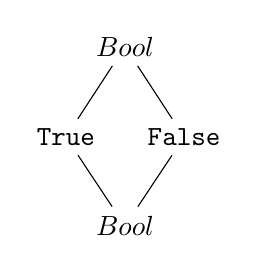
\begin{tikzpicture}[node distance=1.8cm]
  %\draw [help lines, dotted] (-8,1) grid (8,-10);

  %\node(Top)   {$\Top{Value}$};
  %\node(Bot)   [below=6cm of Top] {$\Bot{Value}$};
  %\path node (center) at ($.5*(Top) + .5*(Bot)$) {};
  %\path node (center) at (0,0) {};

  %\path node (bool)    at ([xshift=-4.2cm, yshift= 11.4mm] center) {};
  \path node (bool)    at (0,0) {};
  %\path node (int)     at ([xshift=-0.8cm, yshift= 11.4mm] center) {};
  %\path node (float)   at ([xshift= 2.4cm, yshift= 11.4mm] center) {};
  %\node(None)          at ([xshift= 5.2cm] center) {\texttt{None}};
  %\node(Undefined)     at ([xshift= 5.4cm] center) {\texttt{Undefined}};
  %\path node (list)    at ([xshift= 7.1cm, yshift= 11.4mm] center) {};
  %\node                at ([xshift= 5.8cm] center) {$\cdots$};
  %\path node (sep)     at ([xshift= 7.4cm] center) {};
  %\path node (nparray) at ([xshift= 9.1cm, yshift= 11.4mm] center) {};

  %\node                at ([xshift= 5.3cm, yshift=-3.0cm] center) {Built-ins};
  %\node                at ([xshift= 7.8cm, yshift=-3.0cm] center) {User defined};

  \node(TopBool)  at (bool)                     {$\Top{Bool}$};
  \node(BotBool)  at ([yshift=-22.8mm] TopBool) {$\Bot{Bool}$};
  \node(True)     at ([xshift=-.75cm, yshift=-1.15cm] TopBool)   {\texttt{True}};
  \node(False)    at ([xshift= .75cm, yshift=-1.15cm] TopBool)  {\texttt{False}};
  %\node[ellipse, dotted, draw, thick, fit=(TopBool) (BotBool) (True) (False), inner sep=-3.3mm] {};
  \foreach \x in {True,False} {
    \draw(TopBool) -- (\x);
    \draw(BotBool) -- (\x);
  }
  %\draw(Top) -- (TopBool);
  %\draw(Bot) -- (BotBool);

  %\node(TopInt) at (int)       {$\Top{Int}$};
  %\node(i0)     at ([xshift=-1.5cm, yshift=-1.15cm] TopInt)   {0};
  %\node(i1)     at ([xshift=-.75cm, yshift=-1.15cm] TopInt)   {1};
  %\node(i4232)  at ([xshift=  .3cm, yshift=-1.15cm] TopInt)   {4232};
  %\node(idots)  at ([xshift= 1.5cm, yshift=-1.15cm] TopInt)   {$\cdots$};
  %\node(BotInt)  [below=1.6cm of TopInt]                 {$\Bot{Int}$};
  %\node[ellipse, dotted, draw, thick, fit=(TopInt) (BotInt) (i0) (idots),
  %      inner ysep=-3mm, inner xsep=-5.5mm] {};
  %\foreach \x in {i0,i1,i4232,idots} {
  %  \draw(TopInt) -- (\x);
  %  \draw(BotInt) -- (\x);
  %}
  %\draw(Top) -- (TopInt);
  %\draw(Bot) -- (BotInt);

  %\node(TopFloat)  at (float) {$\Top{Float}$};
  %\node(BotFloat)  at ([yshift=-22.8mm] TopFloat) {$\Bot{Float}$};
  %\node(Float)     at ([yshift=-11.4mm] TopFloat) {\textit{Float}};
  %\draw(Top) -- (TopFloat);
  %\draw(Bot) -- (BotFloat);
  %\node[ellipse, dotted, draw, thick, fit=(TopFloat) (BotFloat), inner sep=-3mm, inner xsep=2mm] {};

  %\draw(Top) -- (None);
  %\draw(Bot) -- (None);

  %\draw(Top) -- (Undefined);
  %\draw(Bot) -- (Undefined);

  % \node(TopList)  at (list) {$\top_{\hspace{-1mm}{\text{\tiny{List}}}}$};
  % \node(BotList)  at ([yshift=-22.8mm] TopList) {$\bot_{\text{\tiny{List}}}$};
  % \node(List)     at ([yshift=-11.4mm] TopList) {\textit{List}};
  % \draw(Top) -- (TopList);
  % \draw(Bot) -- (BotList);
  % \node[ellipse, dotted, draw, thick, fit=(TopList) (BotList), inner sep=-3mm, inner xsep=2mm] {};

  % \node(upsep)    at ([yshift=-3.5cm] sep) {};
  % \node(downsep)  at ([yshift= 3.5cm] sep) {};
  % \draw[dotted, thick](upsep) -- (downsep);

  % \node(TopArray)  at (nparray) {$\top_{\hspace{-1mm}{\text{\tiny{NPArray}}}}$};
  % \node(BotArray)  at ([yshift=-22.8mm] TopArray) {$\bot_{\text{\tiny{NPArray}}}$};
  % \node(List)     at ([yshift=-11.4mm] TopArray) {\textit{NPArray}};
  % \draw(Top) -- (TopArray);
  % \draw(Bot) -- (BotArray);
  % \node[ellipse, dotted, draw, thick, fit=(TopArray) (BotArray), inner sep=-3mm, inner xsep=2mm] {};

\end{tikzpicture}
%\end{preview}
%\end{document}

\end{center}

%\begin{verbatim}
%    Top_{Bool#}
%     /      \
%  True#    False#
%     \      /
%    Bot_{Bool#}
%\end{verbatim}

\begin{quote}
 \textbf{Notation}: Notice that in the figure above\footnote{%
   This kind of diagram is called Hasse diagram. A Hasse indicates the order of the
   elements in a partially ordered set by means of the position of the elements in the
   diagram and the links between them. An element connected to other below is consider
   bigger or equal than the element below.
 }, we abuse notation and write \(\text{False}\) and \(\text{True}\) for the elements
 \(\text{False}^\sharp\) and \(\text{True}^\sharp\), respectively. We have done this to
 keep the equations simple, but strictly speaking the elements from \(\text{Bool}^\sharp\)
 are not interchangeable with the elements of \(\text{Bool}\).
\end{quote}

The Galois connection for this lattice is also quite simple:

\[
\begin{array}{rl}
  \alpha \colon \mathcal{P}(\text{Bool}) &\to \text{Bool}^\sharp \\
  \emptyset       & \mapsto \Bot{Bool} \\
  \{True\}        & \mapsto True^\sharp \\
  \{False\}       & \mapsto False^\sharp \\
  \{True, False\} & \mapsto \Top{Bool} \\
\end{array}
\]

Where \(\gamma{}\) is just defined as \(\alpha^{-1}\) given
\(\alpha{}\)'s bijectivity.

Notice how our previous two Abstract Domains do not require us to define widening or
narrowing operators because none of them has an infinite ascending chain of values, i.e.
there do not exist \(v_i\) for all \(i \in \mathbb{N}\) such that \(v_i \le v_{i+1}\).

For \(\text{Int}\) and \(\text{Float}\) there a pletora of Abstract Domains to chose from.
For an in depth analysis on many of the available Abstract Domains for numbers
see~\textcite{mine_weakly_2004}. We are going to use here the simplest Abstract Domain for
number systems there is: Constant Propagation \autocite{kildall_unified_1973}.

Constant Propagation is very simple, in fact, the previously defined
\(\text{Bool}^\sharp\) Abstract Domain is a Constant Propagation Abstract Domain. We
define \(\text{Int}\)'s Abstract Domain as:

\begin{center}
%\documentclass[12pt,landscape]{article}
%\usepackage{tikz}
%\usetikzlibrary{positioning}
%\usetikzlibrary{fit,shapes.geometric}
%\usetikzlibrary{calc}
%\usepackage{amsfonts}
%\usepackage{amsmath, amsthm, amssymb}
%\usepackage{verbatim}

%\usepackage[active, tightpage]{preview} % used to crop file size to image size
%\setlength\PreviewBorder{0pt}%
%\begin{document}
%\begin{preview}
\begin{tikzpicture}[node distance=1.8cm]
  %\draw [help lines, dotted] (-8,1) grid (8,-10);

  %\node(Top)   {$\Top{Value}$};
  %\node(Bot)   [below=6cm of Top] {$\Bot{Value}$};
  %\path node (center) at ($.5*(Top) + .5*(Bot)$) {};
  %\path node (center) at (0,0) {};

  %\path node (bool)    at ([xshift=-4.2cm, yshift= 11.4mm] center) {};
  %\path node (int)     at ([xshift=-0.8cm, yshift= 11.4mm] center) {};
  \path node (int)    at (0,0) {};
  %\path node (float)   at ([xshift= 2.4cm, yshift= 11.4mm] center) {};
  %\node(None)          at ([xshift= 5.2cm] center) {\texttt{None}};
  %\node(Undefined)     at ([xshift= 5.4cm] center) {\texttt{Undefined}};
  %\path node (list)    at ([xshift= 7.1cm, yshift= 11.4mm] center) {};
  %\node                at ([xshift= 5.8cm] center) {$\cdots$};
  %\path node (sep)     at ([xshift= 7.4cm] center) {};
  %\path node (nparray) at ([xshift= 9.1cm, yshift= 11.4mm] center) {};

  %\node                at ([xshift= 5.3cm, yshift=-3.0cm] center) {Built-ins};
  %\node                at ([xshift= 7.8cm, yshift=-3.0cm] center) {User defined};

  %\node(TopBool)  at (bool)                     {$\Top{Bool}$};
  %\node(BotBool)  at ([yshift=-22.8mm] TopBool) {$\Bot{Bool}$};
  %\node(True)     at ([xshift=-.75cm, yshift=-1.15cm] TopBool)   {\texttt{True}};
  %\node(False)    at ([xshift= .75cm, yshift=-1.15cm] TopBool)  {\texttt{False}};
  %\node[ellipse, dotted, draw, thick, fit=(TopBool) (BotBool) (True) (False), inner sep=-3.3mm] {};
  %\foreach \x in {True,False} {
  %  \draw(TopBool) -- (\x);
  %  \draw(BotBool) -- (\x);
  %}
  %\draw(Top) -- (TopBool);
  %\draw(Bot) -- (BotBool);

  \node(TopInt) at (int)                 {$\Top{Int}$};
  \node(BotInt)  [below=1.6cm of TopInt] {$\Bot{Int}$};
  \node(i0)     at ([xshift=-1.5cm, yshift=-1.15cm] TopInt)   {0};
  \node(i1)     at ([xshift=-.75cm, yshift=-1.15cm] TopInt)   {1};
  \node(i4232)  at ([xshift=  .3cm, yshift=-1.15cm] TopInt)   {4232};
  \node(idots)  at ([xshift= 1.5cm, yshift=-1.15cm] TopInt)   {$\cdots$};
  %\node[ellipse, dotted, draw, thick, fit=(TopInt) (BotInt) (i0) (idots),
  %      inner ysep=-3mm, inner xsep=-5.5mm] {};
  \foreach \x in {i0,i1,i4232,idots} {
    \draw(TopInt) -- (\x);
    \draw(BotInt) -- (\x);
  }
  %\draw(Top) -- (TopInt);
  %\draw(Bot) -- (BotInt);

  %\node(TopFloat)  at (float) {$\Top{Float}$};
  %\node(BotFloat)  at ([yshift=-22.8mm] TopFloat) {$\Bot{Float}$};
  %\node(Float)     at ([yshift=-11.4mm] TopFloat) {\textit{Float}};
  %\draw(Top) -- (TopFloat);
  %\draw(Bot) -- (BotFloat);
  %\node[ellipse, dotted, draw, thick, fit=(TopFloat) (BotFloat), inner sep=-3mm, inner xsep=2mm] {};

  %\draw(Top) -- (None);
  %\draw(Bot) -- (None);

  %\draw(Top) -- (Undefined);
  %\draw(Bot) -- (Undefined);

  % \node(TopList)  at (list) {$\top_{\hspace{-1mm}{\text{\tiny{List}}}}$};
  % \node(BotList)  at ([yshift=-22.8mm] TopList) {$\bot_{\text{\tiny{List}}}$};
  % \node(List)     at ([yshift=-11.4mm] TopList) {\textit{List}};
  % \draw(Top) -- (TopList);
  % \draw(Bot) -- (BotList);
  % \node[ellipse, dotted, draw, thick, fit=(TopList) (BotList), inner sep=-3mm, inner xsep=2mm] {};

  % \node(upsep)    at ([yshift=-3.5cm] sep) {};
  % \node(downsep)  at ([yshift= 3.5cm] sep) {};
  % \draw[dotted, thick](upsep) -- (downsep);

  % \node(TopArray)  at (nparray) {$\top_{\hspace{-1mm}{\text{\tiny{NPArray}}}}$};
  % \node(BotArray)  at ([yshift=-22.8mm] TopArray) {$\bot_{\text{\tiny{NPArray}}}$};
  % \node(List)     at ([yshift=-11.4mm] TopArray) {\textit{NPArray}};
  % \draw(Top) -- (TopArray);
  % \draw(Bot) -- (BotArray);
  % \node[ellipse, dotted, draw, thick, fit=(TopArray) (BotArray), inner sep=-3mm, inner xsep=2mm] {};

\end{tikzpicture}
%\end{preview}
%\end{document}

\end{center}

%\begin{verbatim}
%                  Top^Int
%  _________________|_______________
% /     /     /          \     \    \
% 0     1    -20 ...
% \_____\_____\__________/_____/____/
%                   |
%                  Bot^Int
%\end{verbatim}

\begin{quote}
\textbf{Notation:} Remember that to keep things light, \(n^\sharp\) is represented as \(n\).
\end{quote}

In the same manner as with \(\text{Bool}^\sharp\), we define the Galois
connection as:

\null\hfill
  \begin{minipage}{.35\textwidth}
    \[\begin{array}{rl}
      \alpha \colon \mathcal{P}(\text{Int}) &\to \text{Int}^\sharp \\
      \emptyset &\mapsto \Bot{Int} \\
      \{n\} &\mapsto n \\
      otherwise &\mapsto \Top{Int} \\
    \end{array}\]
  \end{minipage}
  and
  \begin{minipage}{.35\textwidth}
    \[\begin{array}{rl}
      \gamma \colon \text{Int}^\sharp &\to \mathcal{P}(\text{Int}) \\
      \Bot{Int} &\mapsto \emptyset \\
      n &\mapsto \{n\} \\
      \Top{Int} &\mapsto \text{Int} \\
    \end{array}\]
  \end{minipage}
\hfill\null
\\[.6em]

where

\[\text{Int}^\sharp = \text{Int} \cup \left\{ \Top{Int}, \Bot{Int} \right\}\]

%\begin{verbatim}
%Int# = Int U {Top_int, Bot_int}
%\end{verbatim}

We define \(\text{Float}^\sharp\) just in the same way.

Now that we have an Abstract Domain for each primitive value, we can construct an
Abstract Domain for \(\mathbf{PrimVal}\). The idea is simple, as shown in the figure
below, we just define an Abstract Domain that groups all the Abstract Domains for
primitive values together:

\begin{center}
%\documentclass[12pt,landscape]{article}
%\usepackage{tikz}
%\usetikzlibrary{positioning}
%\usetikzlibrary{fit,shapes.geometric}
%\usetikzlibrary{calc}
%\usepackage{amsfonts}
%\usepackage{amsmath, amsthm, amssymb}
%\usepackage{verbatim}

%\usepackage[active, tightpage]{preview} % used to crop file size to image size
%\setlength\PreviewBorder{0pt}%
%\begin{document}
%\begin{preview}
\begin{tikzpicture}[node distance=1.8cm]
  %\draw [help lines, dotted] (-8,1) grid (8,-10);

  \node(Top)   {$\Top{PrimVal}$};
  \node(Bot)   [below=6cm of Top] {$\Bot{PrimVal}$};
  \path node (center) at ($.5*(Top) + .5*(Bot)$) {};

  \path node (bool)    at ([xshift=-4.2cm, yshift= 11.4mm] center) {};
  \path node (int)     at ([xshift=-0.8cm, yshift= 11.4mm] center) {};
  \path node (float)   at ([xshift= 2.4cm, yshift= 11.4mm] center) {};
  \node(None)          at ([xshift= 5.2cm, yshift= 8.4mm] center) {\texttt{None}};
  %\node(Undefined)     at ([xshift= 5.4cm] center) {\texttt{Undefined}};
  %\path node (list)    at ([xshift= 7.1cm, yshift= 11.4mm] center) {};
  %\node                at ([xshift= 5.8cm] center) {$\cdots$};
  %\path node (sep)     at ([xshift= 7.4cm] center) {};
  %\path node (nparray) at ([xshift= 9.1cm, yshift= 11.4mm] center) {};

  %\node                at ([xshift= 5.3cm, yshift=-3.0cm] center) {Built-ins};
  %\node                at ([xshift= 7.8cm, yshift=-3.0cm] center) {User defined};

  \node(TopBool)  at (bool)  {$\Top{Bool}$};
  \node(True)     at ([xshift=-.75cm, yshift=-1.15cm] TopBool)   {\texttt{True}};
  \node(False)    at ([xshift= .75cm, yshift=-1.15cm] TopBool)  {\texttt{False}};
  \node(BotBool)  at ([yshift=-22.8mm] TopBool)                 {$\Bot{Bool}$};
  \node[ellipse, dotted, draw, thick, fit=(TopBool) (BotBool) (True) (False), inner sep=-3.3mm] {};
  \foreach \x in {True,False} {
    \draw(TopBool) -- (\x);
    \draw(BotBool) -- (\x);
  }
  \draw(Top) -- (TopBool);
  \draw(Bot) -- (BotBool);

  \node(TopInt) at (int)       {$\Top{Int}$};
  \node(i0)     at ([xshift=-1.5cm, yshift=-1.15cm] TopInt)   {0};
  \node(i1)     at ([xshift=-.75cm, yshift=-1.15cm] TopInt)   {1};
  \node(i4232)  at ([xshift=  .3cm, yshift=-1.15cm] TopInt)   {4232};
  \node(idots)  at ([xshift= 1.5cm, yshift=-1.15cm] TopInt)   {$\cdots$};
  \node(BotInt)  [below=1.6cm of TopInt]                 {$\Bot{Int}$};
  \node[ellipse, dotted, draw, thick, fit=(TopInt) (BotInt) (i0) (idots),
        inner ysep=-3mm, inner xsep=-5.5mm] {};
  \foreach \x in {i0,i1,i4232,idots} {
    \draw(TopInt) -- (\x);
    \draw(BotInt) -- (\x);
  }
  \draw(Top) -- (TopInt);
  \draw(Bot) -- (BotInt);

  \node(TopFloat)  at (float) {$\Top{Float}$};
  \node(BotFloat)  at ([yshift=-22.8mm] TopFloat) {$\Bot{Float}$};
  \node(Float)     at ([yshift=-11.4mm] TopFloat) {\textit{Float}};
  \draw(Top) -- (TopFloat);
  \draw(Bot) -- (BotFloat);
  \node[ellipse, dotted, draw, thick, fit=(TopFloat) (BotFloat), inner sep=-3mm, inner xsep=2mm] {};

  \node(BotNone)  at ([yshift=-16.8mm] None) {$\Bot{None}$};
  \node[ellipse, dotted, draw, thick, fit=(None) (BotNone), inner sep=-1mm, inner xsep=2mm] {};
  \draw(None) -- (BotNone);
  \draw(Top) -- (None);
  \draw(Bot) -- (BotNone);

  %\draw(Top) -- (Undefined);
  %\draw(Bot) -- (Undefined);

  % \node(TopList)  at (list) {$\top_{\hspace{-1mm}{\text{\tiny{List}}}}$};
  % \node(BotList)  at ([yshift=-22.8mm] TopList) {$\bot_{\text{\tiny{List}}}$};
  % \node(List)     at ([yshift=-11.4mm] TopList) {\textit{List}};
  % \draw(Top) -- (TopList);
  % \draw(Bot) -- (BotList);
  % \node[ellipse, dotted, draw, thick, fit=(TopList) (BotList), inner sep=-3mm, inner xsep=2mm] {};

  % \node(upsep)    at ([yshift=-3.5cm] sep) {};
  % \node(downsep)  at ([yshift= 3.5cm] sep) {};
  % \draw[dotted, thick](upsep) -- (downsep);

  % \node(TopArray)  at (nparray) {$\top_{\hspace{-1mm}{\text{\tiny{NPArray}}}}$};
  % \node(BotArray)  at ([yshift=-22.8mm] TopArray) {$\bot_{\text{\tiny{NPArray}}}$};
  % \node(List)     at ([yshift=-11.4mm] TopArray) {\textit{NPArray}};
  % \draw(Top) -- (TopArray);
  % \draw(Bot) -- (BotArray);
  % \node[ellipse, dotted, draw, thick, fit=(TopArray) (BotArray), inner sep=-3mm, inner xsep=2mm] {};

\end{tikzpicture}
%\end{preview}
%\end{document}

\end{center}

%\begin{verbatim}
%                  Top_primvals
%      _________________|_______________
%     /             /                   \
%   Top_int        Top_float
% ____|____     ____|____
%/  /   \  \   /  /   \  \   Bool  Undefined NoneType
%0  1   ...   .4 nan  ...
%\__\___/__/   \__\___/__/
%     |             |
%   Bot_int        Bot_float
%     \_____________\___________________/
%                       |
%                    Bot_primvals
%\end{verbatim}

The formal definition is in the same lines as the others already shown. Now, consider the
Galois connection:

\[\begin{array}{rl}
  \alpha_{\text{PrimVal}} \colon \mathcal{P}(\text{PrimVal}) &\to \text{PrimVal}^\sharp \\
  \emptyset &\mapsto \Bot{PrimVal} \\
  \{n\} &\mapsto n^\sharp \\
  s &\mapsto \left\{
  \begin{array}{ll}
    \Top{Int} & \text{if } \forall m \in s: m \in \text{Int} \\
    \Top{Float} & \text{if } \forall m \in s: m \in \text{Float} \\
    \Top{Bool} & \text{if } \forall m \in s: m \in \text{Bool} \\
    \Top{PrimVal} & \text{otherwise} \\
  \end{array} \right. \\
\end{array}\]

This is not the only way to define an Abstract Domain out of other Abstract Domains. In
fact, there are many ways, one of which is to define an Abstract Domain where each
individual Abstract Domain is extended with a new \(\undefm_{\text{Type}}\) value, and
they are all grouped into a tuple \autocite{fromherz_static_2018}.

%{\todo{this is lacking a proper proof of the Galois connection property}}

\subsubsection*{\texorpdfstring{\(\mathbf{Val}\)s Abstract
Domain}{Vals Abstract Domain}}\label{vals-abstract-domain}

\noindent \textbf{\(\mathbf{Val}\) definition}

Remember \(\mathbf{Val}\)'s definition:

\vspace*{-1em}
$$\begin{array}{rcl}
  \mathbf{Val} &:=& \mathbf{PrimVal} \alt \mathbf{Object} \alt \textbf{\texttt{<prim-callable>}} \\
         &\alt& \mathbf{Addr} \times \textbf{\texttt{<prim-callable>}} \quad \textit{function associated to value} \\
  \mathbf{Object} &:=& \mathbf{Type} \times \mathbf{Addr} \times \left(\mathbf{Key} \to \mathbf{Addr} \cup \{\undefm\}\right) \\
  \\
  \mathbf{Type} &:=& \texttt{List} \alt \texttt{Tuple} \alt \texttt{Module} \\
  \mathbf{Key} &:=& \mathbf{Iden} + \left(\textsf{string} \times \mathbf{Val}\right) \\
  \\
  \mathbf{Heap}  &:=& \mathbf{Addr} \to \mathbf{Val} \cup \{\undefm\} \\
\end{array}$$

%\begin{verbatim}
%Val = PrimVal | Object | <prim-callable>
%Object = Type x Addr x (Key → Addr + Undefined)
%
%Type = List | Tuple | Module | NdArray
%Key = Iden + (string x (Iden + PrimVal))
%
%Heap = Addr → Val    -- Heap
%\end{verbatim}

A couple of important details about \(\mathbf{Val}\)'s definition:

\begin{itemize}
\tightlist
\item A \(\mathbf{Val}\) can be a \(\mathbf{PrimVal}\), an \(\mathbf{Object}\) or a
  \(\textbf{\texttt{<prim-callable>}}\).
\item A \(\mathbf{Val}\) is not isolated, it makes part of a bigger set of variables, all
  of them must be defined in \(\mathbf{Heap}\). Any \(\mathbf{Val}\) we define must be
  stored in \(\Hea \in \mathbf{Heap}\).
\item We say that a \((a, \Hea) \in \mathbf{Addr} \times \mathbf{Heap}\) is a
  \textbf{valid} value if every value defined in \(\Hea\):
  \(vars = \{v \in Img(\Hea) : v \ne \text{Undefined}\}\) is reachable from
  \(\Hea(a)\), and no \(\mathbf{Addr}\) inside any defined \(\mathbf{Addr}\)
  points to \(\undefm\).
\end{itemize}

An example of a possible value is \((0, \Hea)\) where \(\Hea\) is defined as:
\\[.4em]

\begin{minipage}{.45\textwidth}
  \[\Hea(m) = \left\{
    \begin{array}{ll}
      (\texttt{List}, 0, l) & \text{if } m = 0 \\
      3 & \text{if } m = 1 \\
      \text{None} & \text{if } m = 2 \\
      4 & \text{if } m = 3 \\
      (\texttt{Tuple}, 4, t) & \text{if } m = 4 \\
      0 & \text{if } m = 5 \\
      \undefm & \text{otherwise} \\
    \end{array}
  \right.\]
\end{minipage}
\begin{minipage}{.45\textwidth}
  \[l(i) = \left\{
    \begin{array}{ll}
      1 & \text{if } i = \texttt{'size'} \\
      2 & \text{if } i = (\texttt{'index'}, 0) \\
      3 & \text{if } i = (\texttt{'index'}, 1) \\
      4 & \text{if } i = (\texttt{'index'}, 2) \\
      \undefm        & \text{otherwise} \\
    \end{array}
  \right.\]

  \[t(i) = \left\{
    \begin{array}{ll}
      5   & \text{if } i = \texttt{'size'} \\
      \undefm & \text{otherwise} \\
    \end{array}
  \right.\]
\end{minipage}
\\[.4em]

%\begin{verbatim}
%H = {
%  0: (List, 0, { 'size': 1, ('index', 0): 2, ('index', 1): 3, ('index', 2): 4}),
%  1: 3,
%  2: None,
%  3: 4,
%  4: (Tuple, 4, {'size': 5}),
%  5: 0
%}
%\end{verbatim}

We shall remember this example from a previous subsection (see \ref{reducedsyntaxapp}). This
heap contains the list \pycode|[None, 4, ()]| in memory.

Notice that the values \((1, \Hea)\), \((2, \Hea)\), \ldots{}, and \((5, \Hea)\) are not
considered valid as it is impossible starting from one of them to reach all other values
in the Heap. We will consider only valid values for the rest of the document, which means
that all equations will assume all values and states to be valid. If we were to find a
non-valid value \((n, \Hea)\), we could define a new \((n, \Hea')\) where \(\Hea'\) has
all non-reachable values removed.

\subsubsection*{\(Val^\sharp\) definition}

An Abstract Value is a tuple
\((a, \Hea^\sharp) \in \mathbf(Addr) \times \mathbf(Val)^\sharp\) where:

\vspace*{-1em}
$$\begin{array}{rcl}
  \mathbf{Val}^\sharp &:=& \mathbf{PrimVal}^\sharp \alt \mathbf{Object}^\sharp \alt
  \textbf{\texttt{<prim-callable>}}^\sharp \\
         &\alt& \mathbf{Addr} \times \textbf{\texttt{<prim-callable>}}^\sharp \\
  \mathbf{Object}^\sharp &:=& \mathbf{Type} \times \mathbf{Addr} \times \left(\left(\mathbf{Key} \to \mathbf{Addr} \cup \{\undefm\}\right) \cup \left\{\texttt{ImBot}, \texttt{ImTop}\right\}\right) \\
  \\
  \mathbf{Heap}^\sharp  &:=& \mathbf{Addr} \to \mathbf{Val}^\sharp \cup \{\undefm\} \\
\end{array}$$

%\begin{verbatim}
%Heap# = Addr → Val# + Undefined    -- Abstract Heap
%
%Val# = PrimVal# | Object# | <prim-callable># | Top_Val | Bot_Val
%Object# = Type x Addr x ((Key → Addr + Undefined) + ImTop + ImBot)
%\end{verbatim}

Notice that a \(\mathbf{Val}^\sharp\) requires a Heap to work! Just as
\(\mathbf{Val}\) required it. Some examples of Abstract Values are
\((a, \Hea^\sharp) \in \mathbf{Val}^\sharp \times \mathbf{Heap}^\sharp\) are:

\[\begin{array}{l}
    (0, [0 \mapsto 3]) \qquad (0, [0 \mapsto \Top{Int}]) \qquad
    (0, [0 \mapsto \Bot{Bool}]) \qquad (0, [0 \mapsto \Top{Val}]) \\
    \\
    (0, [\\
    \quad 0 \mapsto (\texttt{List}, 0,
              [\texttt{'size'} \mapsto 1,
              \left(\texttt{'index'}, 0\right) \mapsto 2,
              \left(\texttt{'index'}, 2\right) \mapsto 0
              \left(\texttt{'index'}, 6\right) \mapsto 3
          ]) \\
    \quad 1 \mapsto \Top{Int} \\
    \quad 2 \mapsto 21.3 \\
    \quad 3 \mapsto (\texttt{Tuple}, 3, \texttt{ImBot}) \\
    ]) \\
\end{array}\]

%\begin{verbatim}
%(0, {0: 3})
%(0, {0: Top_Int})
%(0, {0: Bot_Bool})
%(0, {0: Top_Val})
%
%(0, {
%  0: (List, 0, { 'size': 1, ('index', 0): 2, ('index', 1): 3, ('index', 2): 4}),
%  1: Top_Int,
%  2: (Tuple, 2, ImTop),
%  3: 21,
%  4: (Tuple, 4, {'size': 5}),
%  5: Bot_Int
%})
%\end{verbatim}

\begin{quote}
  \textbf{Notation}: Once more, we are abusing notation for convinience. \([]\) represents
  a function which codomain is only \(\undefm\), and
  \([0 \mapsto 5, 1 \mapsto \text{None}]\) represents a function which output to the in
  puts \(0\) and \(1\) is \(5\) and \(\text{None}\), respectively.
\end{quote}

Notice that we can represent any valid value \((a, H^\#)\) as a graph
with \(a\) as root:

%{\inlinetodo{convert nodes below into latex figures}}

%\begin{verbatim}
%({1}, {1: 3}, {(1,1): Undefined}, 1)
%  (3)
%
%-- if a pair (a, b) \in V x V is not shown, then it is Undefined
%({1}, {1: Top_Int}, {}, 1)
%  (Top_Int)
%
%({1}, {1: Top_Bool}, {}, 1)
%  (Bot_Bool)
%
%({1}, {1: Top_Val}, {}, 1)
%  (Top_Val)
%
%(0, {
%  0: (List, 0, { 'size': 1, ('index', 0): 2, ('index', 1): 3, ('index', 2): 4}),
%  1: Top_Int,
%  2: (Tuple, 2, ImTop),
%  3: 21,
%  4: (Tuple, 4, {'size': 5}),
%  5: Bot_Int
%})
%
%({0, 1, 2, 3, 4, 5, 6},
% {0: List,
%  1: Top_Int,
%  2: Top_Tuple,
%  3: 21,
%  4: Tuple,
%  5: Bot_Int,
%  },
%  {(0,1): 'size',
%   (0,2): ('index', 0),
%   (0,3): ('index', 1),
%   (0,4): ('index', 2),
%   (4,5): 'size'
%   },
%   1)
%
%  (List)
%   |-- 'size'       → (Top_Int)
%   |-- ('index', 0) → (Top_Tuple)
%   |-- ('index', 1) → (21)
%   |-- ('index', 2) → (Tuple)
%                        |-- 'size' → (Bot_Int)
%\end{verbatim}

We have defined the first ingredient of the \(\mathbf{Val}^\sharp\) Abstract Domain. The
steps left are:

\begin{itemize}
\tightlist
\item Define abstraction \(\alpha\) and concretisation \(\gamma\) functions,
\item define an order relation,
\item join (\(\sqcup_{\text{Val}^\sharp}\)) and merge (\(\sqcap_{\text{Val}^\sharp}\))
  operations, and
\item a Galois connection.
\end{itemize}

\subsubsection*{\(\sqcup_{\text{Val}^\sharp}\) definition}

We will start by defining the \emph{join} operation and the rationale behind its inner
workings. All other operations and functions are constructed in a very similar way as
\emph{join} is defined.

\begin{verbatim}
Uval: (Addr x Heap#) x (Addr x Heap#) → (Addr x Heap#)
(n, H1#) Uval (m, H2#) :=
  let on := H1#(n)
      om := H2#(m)
   in if on is Object# and om is Object#
      then let (n', joined, Hnew#) := joinVal((n, H1#), (m, H2#), join_empty, H_empty)
            in (n', removeallInConstruction(Hnew#, joined, H1#, H2#))
      else if on is PrimVal# and om is PrimVal#
      then (0, H_empty#[0→on UPrimVal# om])
      else if on = Bot_Val
      then (0, H_empty#[0→om])
      else if om = Bot_Val
      then (0, H_empty#[0→on])
      -- checking all other cases TopVal = TopVal, <prim-_> = <prim-_>, ...
      else if on = om
      then (0, H_empty#[0→on])
      -- the last case is when the two values have different types altogether
      else (0, H_empty#[0→Top_Val])

join_empty: Addr x Addr → (Addr + Undefined)
join_emtpy(a,b) := Undefined

H_empty: Heap#
H_empty(a) := Undefined
\end{verbatim}

\emph{join} revises the type of both values and defines a value that unifies them, they
follow the following sensible rules:

\begin{itemize}
\tightlist
\item \(\Bot{Val}\) must be the lowest value in the order, therefore any value joining
  with it should be the same value (\(\Bot{Val} \sqcup n = n\)).
\item \(\Top{Val}\) is the biggest value in the order, therefore any value joining with it
  should give back \(\Top{Val}\) (\(\Top{Val} \sqcup n = \Top{Val}\)).
\item Values of the same kind, \(\mathbf{PrimVal}^\sharp\), \(\mathbf{Object}^\sharp\) and
  \(\textbf{\texttt{<prim-callable>}}^\sharp\), should not be comparable, e.g.~any value
  from \(\mathbf{PrimVal}^\sharp\) joined with any of \(\mathbf{Object}^\sharp\) should
  gives \(\Top{Val}\).
\item Joining \(\mathbf{PrimVal}^\sharp\)s should use \(\sqcup_{\text{PrimVal}^\sharp}\).
\item Joining \(\mathbf{Object}^\sharp\)s should take into account the recursive nature of
  the definition of \(\mathbf{Val}^\sharp\)s and \(\mathbf{Object}^\sharp\)s.
\end{itemize}

Without further ado, the definition of \(\sqcup_{\text{Val}^\sharp}\) (\pycode|joinVal|):

\begin{verbatim}
HeapCon# = Addr → Val# + Undefined + InConstruction

-- we assume that (n,H1#) and (n,H1#) are Object#s
joinVal: (Addr x Heap#) x (Addr x Heap#) x (Addr x Addr → Addr + Undefined) x HeapCon#
       → Addr x (Addr x Addr → Addr + Undefined) x HeapCon#
joinVal((n,H1#), (m, H2#), joined, H_new#) :=
  let joined_left := {l \in Addr | E r \in Addr : joined(l,r) != Undefined}
      joined_right := {r \in Addr | E l \in Addr : joined(l,r) != Undefined}

   in if n in joined_left or m in joined left -- n or m has already been visited
      then  if joined(n, m) != Undefined
            -- an address for the new Object# has already been defined
            then (joined(n,m), joined, H_new#)
            -- either n or m had already been joined to another object, every variable
            -- they can reach should be Top_Val because the paths to reach them are
            -- different in the two states
            else let (joined', H_new'#) :=
                           makeallreachabletop((n, H1#), (m, H2#), joined, H_new#)
                     ad := freeaddr(H_new'#)
                  in (ad, joined[(n,m)→add], H_new'#[ad→Top_Val])
      -- we know that H1#(n) and H2#(m) are both 'Object#'s because the call from UVal#
      -- checked so
      else let -- n and m haven't already been visited
             (tn, adn, fn) := H1#(n)
             (tm, adm, fm) := H2#(m)
        in if tn != tm -- the two Object#s are not of the same type
           then let (joined', H_new'#) :=
                          makeallreachabletop((n, H1#), (m, H2#), joined, H_new#)
                    ad := freeaddr(H_new'#)
                 in (ad, joined[(n,m)→add], H_new'#[ad→Top_Val])
           -- both objects have the same type
           else if fn = ImTop and fm = ImTop
                then let ad := freeaddr(H_new'#)
                      in (ad, joined[(n,m)→ad], H_new#[ad→(tn,ad,ImTop)])
                else if fn = ImTop
                then let (joined', H_new'#) :=
                               makeallreachabletop_right((m, H2#), joined, H_new#)
                         ad := freeaddr(H_new'#)
                      in (ad, joined'[(n,m)→ad], H_new'#[ad→Top_Val])
                else if fm = ImTop
                then let (joined', H_new'#) :=
                               makeallreachabletop_left((n, H1#), joined, H_new#)
                         ad := freeaddr(H_new'#)
                      in (ad, joined'[(n,m)→ad], H_new'#[ad→Top_Val])
                -- if any of the two values is Bot then we leave the new value as
                -- InConstruction until the end of the execution
                else if fn = ImBot or fm = ImBot
                then let adnew := freeaddr(H_new#)
                      in (adnew, joined[(m,n)→adnew], H_new#[adnew→InConstruction])
                -- both, fn and fn, are (Key → Addr + Undefined)
                -- notice that `InConstruction` is assigned to the address `ad`, but
                -- once we return from the recursive call we can now replace the value
                -- for a proper object definition
                else let ad := freeaddr(H_new#)
                         (fnew, joined', H_new'#) := joinObjectFn(
                                                        (fn, H1#),
                                                        (fm, H2#),
                                                        joined[(n,m)→ad],
                                                        H_new#[ad→InConstruction])
                      in if H_new'#(ad) = InConstruction
                         then (ad, joined', H_new'#[ad→(nt, ad, fnew)])
                         else (ad, joined', H_new'#)

joinObjectFn: ((Key → Addr + Undefined) x Heap#) x ((Key → Addr + Undefined) x Heap#)
            x (Addr x Addr → Addr + Undefined) x HeapCon#
            → (Key → Addr + Undefined) x (Addr x Addr → Addr + Undefined) x HeapCon#
joinObjectFn((fn, H1#), (fm, H2#), joined, H_new#) :=
   let fn_empty: (Key → Addr + Undefined)
       fn_empty = Undefined

       PreIm: (Key → Addr + Undefined) → P(Key)
       PreIm(fun) := {ad \in Addr | fun(ad) != Undefined}

       helper: ((Key → Addr + Undefined) x (Addr x Addr → Addr + Undefined) x HeapCon#)
               x Key
               → ((Key → Addr + Undefined) x (Addr x Addr → Addr + Undefined) x HeapCon#)
       helper((fnew, joined, H_new#), key) :=
         if fm(key) = Undefined
         then let (joined', H_new'#) :=
                        makeallreachabletop_left((fn(key), H1#), joined, H_new#)
                  ad := freeadd(H_new'#)
               in (fnew[key→ad], joined', H_new'#[ad→Top_Val])
         else if fn(key) = Undefined
         then let (joined', H_new'#) :=
                        makeallreachabletop_right((fm(key), H2#), joined, H_new#)
                  ad := freeadd(H_new'#)
               in (fnew[key→ad], joined', H_new'#[ad→Top_Val])
         -- key is defined in both, fn and fm
         else let
            adn := fn(key)
            adm := fm(key)
            val1 := H1#(adn)
            val2 := H2#(adm)
            ad := freeadd(H_new'#)

         -- same code that was in
         in if val1 is Object# and val2 is Object#
            then let (n', joined', H_new'#) = joinVal((n, H1#), (m, H2#), joined, H_new#)
                  in (fnew[key→n'], joined', H_new'#)
            else if val1 is PrimVal# and val2 is PrimVal#
            then (fnew[key→ad], joined[(adn,adm)→ad], H_new#[ad→val1 UPrimVal# val2])
            else if on = Bot_Val
            then (fnew[key→ad], joined[(adn,adm)→ad], H_new#[ad→InConstruction])
            else if val2 = Bot_Val
            then (fnew[key→ad], joined[(adn,adm)→ad], H_new#[ad→InConstruction])
            -- checking all other cases TopVal = TopVal, <prim-_> = <prim-_>, ...
            else if on = val2
            then (fnew[key→ad], joined[(adn,adm)→ad], H_new#[ad→on])
            -- the last case is when the two values have different types altogether
            else (fnew[key→ad], joined[(adn,adm)→ad], H_new#[ad→Top_Val])

    in foldl(helper, (fn_emtpy, joined, H_new#), PreIm(fn) U PreIm(fm))
\end{verbatim}

% {\inlinetodo{there are a couple of functions missing, one of them is
% \pycode|makealltop|}}

Notice that it is in \pycode|joinVal| (\(\sqcup_{\text{Val}^\sharp}\)) where the whole
magic of this Abstract Domain lies. \pycode|joinVal| is meant to walk through both graphs
simultaneously, find the similarities, implode the differences between the graphs and
preserve all parts that coincide.

The definition of \pycode|joinVal| requires the help of the function \pycode|joinObjectFn|
which joins the values to which an \(\mathbf{Object}^\sharp\) points (the function
\(\left(\mathbf{Key} \to \mathbf{Addr} \cup \{\undefm\}\right)\)).

\pycode|joined| is a function that stores the similarities between nodes
(values), and \pycode|Hnew#| stores the values of each new value. The
type of \pycode|Hnew#| is not \(\Hea^\sharp\) but
\(\mathbf{Addr} \to \mathbf{Val}^\sharp \cup \{\undefm, \mathsf{InConstruction}\}\), i.e.
the output of \pycode|Hnew#| is the same of \(\Hea^\sharp\) but it has an additional value
called \pycode|InConstruction|. The new value to which a heap can point to is
\pycode|InConstruction| and it is meant to be a wildcard value while the graph is being
constructed.

% {\inlinetodo{Reconsider eliminating the whole paragraph from below: We
% will never see a Bottom value in Pytropos, as the only way for it to
% appear would be to \emph{merge} two values, but that is never going to
% happen as \emph{merge} was not defined because there is never a use for
% it (the only way to use \emph{merge} would be by incoporating backward
% assignment, which is out of the scope of Pytropos)}}

One last function, that was not explained before is
\pycode|removeallInConstruction|. It is in charge of looking in the Heap
if there is any reference to some \pycode|InConstruction| value left.
All \pycode|InConstruction| values left after returning from the whole
walk will only be those which appeared when joining some node to a
\(\texttt{ImBot}\) or \pycode|Bot_Val|. Because we expect
\(\texttt{ImBot} \sqcup fn = fn\), we must copy all values from the joining
heaps into the new heap.

%\inlinetodo{Fill section with examples}
%Because the \enquote{code} describing how to \emph{join} to abstract
%values can be rather coarse, we present to you the algorithm working in
%a couple of examples. The two graphs at the left represent the two
%values to join, on the right the resulting new value is defined.

% {\inlinetodo{show six examples of uniting different values, they can be
% as complicated as possible. \texttt{1 U 2},
% \texttt{[1,2]\ U\ [1,3]},
% \texttt{a = [2, 3]; a.append(a)} (extract three more examples
% from tests)}}

% {\inlinetodo{Add note saying that this scheme of Abstract Domain is
% general enough to let us switch between different non-relation Abstract Domain for
% the PrimVals. There are probably some tweaks necessary to allow this Abstract Domain
% to work with relational Abstract Domains for the PrimVals}}

\subsubsection*{\(\mathbf{Val}^\sharp\) Order definition}

Now that we have defined the \emph{join} function, we can move to the
function that defines a lattice, the order function.

We define \(\le\) as \(a \le_{\text{Val}^\sharp} b \iff b = a \sqcup_{\text{Val}^\sharp} b\).
This definition follows from the definition of \emph{join}: given any two values
\(a,b \in\) lattice, it is always possible to find a value that is bigger than \(a\) and
\(b\) such that it is the smallest of the bigger values. In the case \(a < b\), then we
can be certain that \(b\) will be the result of \emph{join}ing \(a\) with \(b\), otherwise
there would be a value smaller than \(b\) that is also bigger or equal than \(b\). What we
are trying to argue in here is that we can define a lattice by either defining an order
relation or a proper \emph{join} operation for it. We leave the proof that \(\le\)
defines an order for valid values
(\((a, \Hea^\sharp) \in \mathbf{Val}^\sharp \times \mathbf{Heap}^\sharp\)) for future
work.

\subsubsection*{Other definitions}

Our goal is not to present in detail all functions and operations necessary to define the
Abstract Domain for \(\mathbf{Val}^\sharp\)s. That would require three times the space
already used in this document. What we wanted to show here is the rationale behind the
implementation to give it a little more formal depth.

The \emph{merge} operation is defined as it was \emph{join}. The main difference between
the two is what is the result of operating two values of different types. \emph{Join}ing
values with differing types gives us \(\top\) values, while \emph{merg}ing gives us
\(\bot\) values.

\subsection{State Abstract Domain}\label{state-abstract-domain-1}

Now that we have a Value Abstract Domain, we can extend it to the State
of a Program. Doing so it's surprisingly easy, as all the blocks have
already been laid down by the Value Abstract Domain.

The State Abstract Domain is defined as the tuple
\texttt{(Global\#,\ Heap\#)} where:

\vspace*{-1em}
\[\begin{array}{rcl}
  \mathbf{Global}^\sharp  &:=& \mathbf{Iden} \to \mathbf{Addr} \cup \{\undefm\} \\
  \mathbf{Heap}^\sharp  &:=& \mathbf{Addr} \to \mathbf{Val}^\sharp \cup \{\undefm\} \\
\end{array}\]

%\begin{verbatim}
%-- Global
%Global# = Iden → Addr + Undefined  -- Abstract Global Scope
%-- Heap
%Heap# = Addr → Val# + Undefined    -- Abstract Heap
%\end{verbatim}

Notice that \(\mathbf{Global}^\sharp\) is a function that takes an identifier and outputs
an address to where the variable is stored, which is just the same thing to what the function
\(\left(\mathbf{Key} \to \mathbf{Addr} \cup \{\undefm\}\right)\) inside
\(\mathbf{Object}^\sharp\) does. In fact, the function inside \(\mathbf{Object}^\sharp\)
has a bigger pre-image than that of \(\mathbf{Global}^\sharp\) (\(\mathbf{Key}\) is
defined as \(\mathbf{Iden} + \left(\textsf{string} \times \mathbf{Val}\right)\)). This
means that we have no need to define a \emph{join} operation from scratch for the State
Abstract Domain. We can just borrow/repurpose the already defined function
\texttt{joinObjectFun}, defined for \(\mathbf{Object}^\sharp\)s to
\(\mathbf{Global}^\sharp\)s!

\begin{verbatim}
UState: (Global#, Heap#) x (Global#, Heap#) → (Global#, Heap#)
(G1#, H1#) UState (G2#, H2#) :=
  let (Gnew#, joined, Hnew#) = joinObjectFn((G1#, H1#), (G2#, H2#), joined_empty, H_empty)
   in (Gnew#, Hnew#)
\end{verbatim}

Similarly, all other functions and operations can be defined as a special
case of the Value Abstract Domain.

\subsection{Abstract Semantics}\label{abstract-semantics-1}

In this section, we present some examples of the abstract semantics.
Notice that we do not need the abstraction and concretisation
functions as the State and State Abstract Domains are quite similar. It
is left for future work to prove that the definitions stated in here are
in fact derived from the Galois connection.

As examples, consider the semantics of expressions:

\begin{verbatim}
E#[expr] : Global# x Heap#
         → Global#
          x Heap#
          x (Val# + (Object# x (string x Val#)) + Iden)

E#[Name(id, ctx)](G#, H#) :=
  match ctx in
    case Load  → if G#(id) = Undefined
                  -- the variable `id` has not been defined then we "set" it in the
                  -- global scope and return `Top_Val`
                  then let ad := freeaddr(H#)
                        in (G#[id→ad], H#[ad→Top_Val], Top_Val)
                  else (G#, H#, G#(id))
    case Store → (G, H, id)
    case Del   → (G, H, id)

E#[BinOp(op, a, b)](G#, H#) :=
  let (G1#, H1#, v1) := E#[a](G#, H#)
      (G2#, H2#, v2) := E#[b](G1#, H1#)
      -- TODO: careful with the two notations you are using to make sure a var is Val#
      --        kind(v) = Val#  vs  isvalue#(v)
   in if kind(v1) ≠ Val#  or  kind(v1) ≠ Val#
      -- Bad parsing! `E[e](G, H)` for e in {a,b} are supposed to return Val#
      -- Parsing errors halt the execution of the Abstract Interpreter
      then <Execution Halt>
      else
        let prim_op# := get_prim_op#(op, v1, v2)
         in prim_op#(G2#, H2#)

get_prim_op : Op x Val# x Val# → Global x Heap → Global x Heap x Val#

get_prim_op#(Add, v1, v2) :=
  match (type(v1), type(v2)) in
    case (Int, Int) → λ(G#, H#) → <prim-+-int>#(v1, v2, G#, H#)
    case (Float, Float) → λ(G#, H#) → <prim-+-float>#(v1, v2, G#, H#)
    case (Int, Bool) → λ(G#, H#)→ <prim-+-int>#(v1, Int(v2), G#, H#)
    case (Bool, Int) → λ(G#, H#)→ <prim-+-int>#(Int(v1), v2, G#, H#)
    case (Float, a) → if a = Bool or a = Int
                       then λ(G#, H#)→ <prim-+-float>#(v1, Float(v2), G#, H#)
                       else <prim-ret-top>#
    case (a, Float) → if a = Bool or a = Int
                       then λ(G#, H#)→ <prim-+-float>#(Float(v1), v2, G#, H#)
                       else <prim-ret-top>#
    case otherwise → <prim-op-top>#

<prim-op-top># : Global# x Heap#
<prim-op-top>#(G#, H#) := (G#, H#, Top_Val)
\end{verbatim}

Notice that parsing errors still halt the execution of the Abstract
Interpreter. It could be possible to work around those errors too, but
parsing errors is out of the scope of the Abstract Interpreter as they hint
to an external problem. We assume that a piece of code is parsed
properly before starting the execution of the code (just as Python
does).

Every function defined in the concrete semantics must be rewritten as function that
operates in the Abstract Domain. For example, consider the function \verb|<prim-+-int>|,
which is defined as:

\verb|<prim-+-int<(i, j, G, H) := (G, H, i+j)|

We need to define its Abstract Interpretation counterpart:

\begin{verbatim}
<prim-+-int>#(i, j, G#, H#) :=
  if i = Top_Int or j = Top_Int
  then (G#, H#, Top_Int)
  else if i = Bot_Int or j = Bot_Int
  then (G#, H#, Bot_Int)
  else (G#, H#, i+j)
\end{verbatim}

And as an example for the semantics of statements consider:

\begin{verbatim}
S#[Assign(var, val)](G#, H#) :=
  let (G1#, H1#, ass) := E[var](G#, H#)
      (G2#, H2#, rightval) := E[val](G1#, H1#)
      -- Parsing error, probably. `rightval` must be a `Val#` if the parsing made no
      -- mistake
      rval := if is_value#(rightval) then val else <Execution Halt>
   in
      match ass in
        case Iden → (G2#[ass→rval], H2#)

        case ((t, addr, o): Object#, ('index', val: PrimVal#)) →
          let setindex# := get_prim_set_index#(t)
          in setindex#(G2#, H2#, o, val, addr, rval)

        -- Parsing error probably. This should never have happened
        otherwise → <Execution Halt>

S#[Import(name)](G#, H#) :=
  let freeaddr := get_free_addr(H#)
   in
     match name in
       ("numpy",) →
         let (Module, arr, mod) := <numpy-mod>
         in  (G#['numpy'→freeaddr], H#[freeaddr→(Module, freeaddr, mod)])
       ("numpy", alias) →
         let (Module, arr, mod) := <numpy-mod>
         in  (G#[alias→freeaddr], H#[freeaddr→(Module, freeaddr, mod)])

       ("pytropos.hints.numpy",) →
          (G#["pytropos.hints.numpy"→freeaddr],
           H#[freeaddr→(Module, freeaddr, <numpy-hints>)])
       ("pytropos.hints.numpy", alias) →
          (G#[alias→freeaddr], H#[freeaddr→(Module, freeaddr, <numpy-hints>)])

       (nm,) →
          (G#[nm→freeaddr], H#[freeaddr→(Module, freeaddr, ImTop)])

       (nm,alias) →
          (G#[alias→freeaddr], H#[freeaddr→(Module, freeaddr, ImTop)])

S[AnnAssign(var, hint, val)](G, H) :=
  let (G1, H1, evaluatedhint) := E[hint](G, H)
      (G2, H2, evaluatedhint) := E[hint](G1, H1)
      hintval := if isvalue#(evaluatedhint) then evaluatedhint else <Execution Halt>

   in S[Assign(var, val)](G1, H1)

  let (G1, H1, ass) := E[var](G, H)
      (G2, H2, evaledhint) := E[hint](G1, H1)
      (G3, H3, rightval) := E[val](G2, H2)
      compval := if is_value(rightval) then val else <Execution Halt>
      hintval := if isvalue#(evaledhint) then evaledhint else <Execution Halt>

      -- if `hintval` is more precise than `compval` we replace it
      rval := if hintval < compval then hintval else compval
   in
      ... -- Continue as in S[Assign(...)]
\end{verbatim}
